\documentclass[a4paper,twoside,11pt]{article}
\usepackage[utf8]{inputenc}
\usepackage{wrapfig}
\usepackage{subcaption}
\usepackage{amsmath,amsthm,array} 
\usepackage{multicol}
\usepackage{adjustbox}
\usepackage{multirow}
\usepackage{longtable}
\usepackage{gensymb}
\usepackage{supertabular}
\usepackage{url}
\usepackage{graphicx}
\usepackage{lipsum}
\usepackage[english]{babel}
\usepackage{fancyhdr}
\usepackage{caption}
\usepackage{blindtext}
\usepackage{lastpage}
\usepackage{titlesec}
\usepackage{hyperref}
\usepackage[resetfonts]{cmap}
\usepackage{fancyvrb}
\begin{VerbatimOut}{ot1.cmap}
%!PS-Adobe-3.0 Resource-CMap
%%DocumentNeededResources: ProcSet (CIDInit)
%%IncludeResource: ProcSet (CIDInit)
%%BeginResource: CMap (TeX-OT1-0)
%%Title: (TeX-OT1-0 TeX OT1 0)
%%Version: 1.000
%%EndComments
/CIDInit /ProcSet findresource begin
12 dict begin
begincmap
/CIDSystemInfo
<< /Registry (TeX)
/Ordering (OT1)
/Supplement 0
>> def
/CMapName /TeX-OT1-0 def
/CMapType 2 def
1 begincodespacerange
<00> <7F>
endcodespacerange
8 beginbfrange
<00> <01> <0000>
<09> <0A> <0000>
<23> <26> <0000>
<28> <3B> <0000>
<3F> <5B> <0000>
<5D> <5E> <0000>
<61> <7A> <0000>
<7B> <7C> <0000>
endbfrange
40 beginbfchar
<02> <0000>
<03> <0000>
<04> <0000>
<05> <0000>
<06> <0000>
<07> <0000>
<08> <0000>
<0B> <0000>
<0C> <0000>
<0D> <0000>
<0E> <0000>
<0F> <0000>
<10> <0000>
<11> <0000>
<12> <0000>
<13> <0000>
<14> <0000>
<15> <0000>
<16> <0000>
<17> <0000>
<18> <0000>
<19> <0000>
<1A> <0000>
<1B> <0000>
<1C> <0000>
<1D> <0000>
<1E> <0000>
<1F> <0000>
<21> <0000>
<22> <0000>
<27> <0000>
<3C> <0000>
<3D> <0000>
<3E> <0000>
<5C> <0000>
<5F> <0000>
<60> <0000>
<7D> <0000>
<7E> <0000>
<7F> <0000>
endbfchar
endcmap
CMapName currentdict /CMap defineresource pop
end
end
%%EndResource
%%EOF
\end{VerbatimOut}
\usepackage[margin=0.7in]{geometry}
\numberwithin{equation}{section}
\pagestyle{fancy}
\fancyhf{}
\rhead{\includegraphics[width=0.04\textwidth]{Stargazing_Mumbai_LOGO1.jpg}}
\lhead{Basics of Astronomy}
\cfoot{\thepage-\pageref{LastPage}}
\rfoot{Email: stargazingmumbai@gmail.com}
\lfoot{Web: stargazingmumbai.in}
\newcommand\sun{\cdot}
\newcommand{\solmas}{\(\textup{M}_\odot\)}

\titleclass{\subsubsubsection}{straight}[\subsection]

\newcounter{subsubsubsection}[subsubsection]
\renewcommand\thesubsubsubsection{\thesubsubsection.\arabic{subsubsubsection}}
\renewcommand\theparagraph{\thesubsubsubsection.\arabic{paragraph}} % optional; useful if paragraphs are to be numbered

\titleformat{\subsubsubsection}
  {\normalfont\normalsize\bfseries}{\thesubsubsubsection}{1em}{}
\titlespacing*{\subsubsubsection}
{0pt}{3.25ex plus 1ex minus .2ex}{1.5ex plus .2ex}

\makeatletter
\renewcommand\paragraph{\@startsection{paragraph}{5}{\z@}%
  {3.25ex \@plus1ex \@minus.2ex}%
  {-1em}%
  {\normalfont\normalsize\bfseries}}
\renewcommand\subparagraph{\@startsection{subparagraph}{6}{\parindent}%
  {3.25ex \@plus1ex \@minus .2ex}%
  {-1em}%
  {\normalfont\normalsize\bfseries}}
\def\toclevel@subsubsubsection{4}
\def\toclevel@paragraph{5}
\def\toclevel@paragraph{6}
\def\l@subsubsubsection{\@dottedtocline{4}{7em}{4em}}
\def\l@paragraph{\@dottedtocline{5}{10em}{5em}}
\def\l@subparagraph{\@dottedtocline{6}{14em}{6em}}
\makeatother

\setcounter{secnumdepth}{4}
\setcounter{tocdepth}{4}

\title{\includegraphics[width=0.25\textwidth]{Stargazing_Mumbai_LOGO1.jpg} \\ Basics of Astronomy}
\author{SM Team}








\begin{document}
\maketitle
\tableofcontents
\newpage
\section{Basics of Stargazing.}
\paragraph{}
A small disclaimer that one might have to keep in mind before we start would be to understand that astronomy is a huge field of study. This originated when the scientific method met astrology. Astronomy has several branches, some of them being, astrophysics, astrochemistry, astrobiology, astrometry etc. We would get into these topics in due time.

\subsection{What are the coordinate systems?}
\paragraph{}
You're an astronomer, and you have discovered a very interesting source in the sky and you need to tell the community about your discovery. The first step to this would be to tell them it's location in the sky. The art (yes, it's an art) of finding the exact location of an object in the sky is called \textbf{astrometry}. It is one of the most important things in astronomy, and hence has it's own field of study. However, before we can dive into astrometry, you need to know what are the systems available to you and which ones should you use and how. The following would be a brief run down (without much of it's history) of the available systems. I would highly recommend that you go through these and go through the page cited in \cite{astrometry_wiki}. 
\subsubsection{Altazimuth Coordinate system}
\begin{wrapfigure}{l}{0.5\textwidth}
\includegraphics[width=0.9\linewidth]{fig1.png} 
\caption{Altitude and Azimuth measurement \\ Image source \cite{azimuth_wiki}}
\label{fig1}
\end{wrapfigure}
\paragraph{}
The name, Altazimuth is actually the combination of the two axes, namely \textbf{Altitude} and \textbf{Azimuth}. The altitude angle is the angle that says how high the object is in the sky from the horizon. So with this definition, the point right above our head will be at 90$\degree$ altitude. This point is called the \textbf{zenith}. The horizon is at 0$\degree$ altitude, and anything in between that is above the horizon is from 0$\degree$ to +90$\degree$. Also, the point right below us, called the \textbf{Nadir} is at -90$\degree$. Sometimes the zenith is used instead of altitude angle, and hence is referred to as the \textbf{zenith angle}, which is basically a complement to the altitude angle. The other angle that helps pin point the object at a certain location, at a given time, is the Azimuth angle. To get this we first join the north and south poles, and then the angle moving from north-east-south-west-north is the azimuth angle. This might be a bit ambiguous, but then the figure \ref{fig1} should clear things out. Hence, to put things into perspective, north to east is 90$\degree$ azimuth, north-east-south is 180$\degree$ azimuth, and north-east-south-west is 270$\degree$ azimuth. North to north would be 360$\degree$. The reverse gives us degrees in negatives. 
\paragraph{}
Now, a few things that one would have to keep in mind is the radius of the sphere in figure \ref{fig1}, is 5 Km, hence if we have a radius of greater than 5 Km then the curvature of the earth would skew the altitude measurements. This also means that this coordinate system is highly location specific. Also, since the earth rotates, the coordinates of any object changes through the night, and hence when communicating the location of any event in the sky, we would have to give our location of observation, the time of observation and the location of the object in the sky during that time. This obviously is too much work, and hence is prone to errors. To avoid these and many other issues, the equatorial coordinate system is used. To know more about azimuth, read through it's wiki page \cite{azimuth_wiki} and \cite{coord_wiki}.
\subsubsection{Equatorial Coordinate system}
\begin{wrapfigure}{l}{0.5\textwidth}
\includegraphics[width=0.9\linewidth]{fig2.png} 
\caption{Equitorial Coordinate system \\ Image source \cite{equi_coord1}}
\label{fig2}
\end{wrapfigure}
\paragraph{}
Now, we know the latitudes and longitudes on earth, and how they form a grid. The equatorial coordinate system is just the projection of this coordinate system into the celestial sphere. Hence \textbf{latitude becomes declination and longitude becomes right ascension}. This kind of coordinate system has the celestial north pole set as the north, that is, as shown in the figure \ref{fig2}. 
\paragraph{}
Now, one might notice that the declination can be easily calculated since that is essentially how high the source is from the celestial equator (which is essentially a projection of the equator on the celestial sphere). However, in order to find the right ascension we need a reference celestial longitude which would be 0 hour. The line we use as a reference is the \textbf{vernal equinox} which is considered to be at 0 hour. 
\paragraph{}
Now, one might be confused as to what do I mean by \textbf{vernal equinox}, how did I get that line, are there any other points of importance in the celestial sphere? The answer to all those questions is yes. Now, before we get into vernal equinox, and what it signifies we need to modify the figure \ref{fig2} a bit. Now, one might know that there is a tilt in the earth's axis, (of roughly \textbf{23.5$\degree$}). This tilt causes the sun's light to fall on earth differently throughout the day, meaning when the southern hemisphere is towards the sun, the northern hemisphere undergoes shorter days, and longer nights, that is winter season (imagine the earth rotating all the while being tilted and the sun's light coming from the left). The opposite happens in case of the southern hemisphere, that is, it has longer days, and shorter nights, in short summer season.
\begin{wrapfigure}{r}{0.5\textwidth}
\begin{center}
\includegraphics[width=0.8\linewidth]{fig3.png} 
\caption{Equatorial coordinate system with ecliptic \\ Image source \cite{equi_coord2}}
\label{fig3}
\end{center}
\end{wrapfigure}
\newpage
\paragraph{}
Now, given that the earth rotates, we have the light from the sun rotating through this tilt. Hence, when we started off this explanation, we considered the sun's light from the left, now we move the earth to the opposite part of it's orbit so that we have the sun light coming from the right of figure \ref{fig2}. This is when the northern hemisphere has summer season, and the southern hemisphere has winter at a given time of a year.
\paragraph{}
Now, if we map this position of the sun throughout the year, into the celestial sphere, we get the line called the \textbf{ecliptic}. Refer the figure \ref{fig3}. Now, we see that once we map this, we have two points that intersects with the celestial equator. 
These points of intersection are those where the day and night are equal (no matter where you are on earth). These points of equal days and nights are called equinoxes. 
\paragraph{}
There are two equinoxes, namely, \textbf{vernal equinox} (the time of the year being \textbf{21$^{st}$ March}) when the sun is traveling from southern hemisphere of the celestial sphere to the northern hemisphere, and, \textbf{autumnal equinox} (the time of the year being \textbf{22$^{nd}$ September}) when the sun is traveling from northern hemisphere of the celestial sphere to the southern hemisphere. 
\paragraph{}
Since the sun travels to the northern hemisphere in March, one can say that vernal equinox marks the beginning of the summer season in the northern hemisphere. And when it exits the northern hemisphere in September, it marks the beginning of the winter season for the northern hemisphere.
\paragraph{}
Now, the other two extremes, as shown in figure \ref{fig3}, are the Solstices, that is, the \textbf{winter and the summer solstices}. These points are the points of extremities in the path of the sun through the sky. These are those periods of the year when the day and light length are at the extremes. The \textbf{winter solstice (22$^{nd}$ December)} is that day in the northern hemisphere that has the shortest day and the longest night. The opposite is true for \textbf{summer solstice (21$^{st}$ June)} when, in the northern hemisphere, the day is the longest. 
\paragraph{NOTE: The equatorial coordinate system is the standard system}
\subsubsection{Ecliptic coordinate system}
\paragraph{}
Now, another similar, but not so widely used, coordinate system is the ecliptic coordinate system that considers the ecliptic as the fundamental plane (equator). The poles become the ecliptic poles and declination becomes ecliptic latitude and right ascension becomes ecliptic longitude. One can go through their wiki page for further details. However, one thing that remains constant is the role of vernal equinox in deciding 0 hours for both the systems.
\subsubsection{Galactic coordinate system}
\paragraph{}
This is the coordinate system that takes the galactic plane as the fundamental plane. This is sometimes used when one wants to map the distribution of globular clusters (we will come to those later) around our galaxy, or when someone wants to plot the locations of the nearby galaxies so that one can visualize the distribution of the galaxies within the local cluster. It's just that the calculation becomes easier with this coordinate system.
\newpage \clearpage
\subsection{What are Epochs?}
\paragraph{}
\begin{wrapfigure}{r}{0.5\textwidth}
\begin{center}
\includegraphics[width=0.5\linewidth]{fig4.png} 
\caption{Precession of the earth's axis pt.1 \\ Image source \cite{precession1}}
\label{fig4}
\end{center}
\end{wrapfigure}
An important point that I would like to add is the concept of \textbf{epoch}, I am not sure how useful this could be for outreach, however, for those of you who are planning to have a career in astrophysics or astronomy would need to know this concept as soon as possible. Now, along with the earth rotating along its rotation axis, and it's revolution around the sun, the earth also precesses around it's rotation axis. Something like that shown in figure \ref{fig4}. The rotation axis rotates around a central axis with a period of $\approx$26000 years (refer \cite{precession1} and \cite{precession3}). Since this happens, over a span of 26000 years, the celestial north pole changes over this time period, since as the axis changes it's direction, so will the north pole change. Right now it is pointing at polaris, however, after $\approx$ 13000 years it would point at the opposite direction nearby Vega, making it our new pole star. 
\paragraph{}
Now, this also means one thing, since the axis changes direction with time, the celestial equator changes as well. This in turn changes the declination and hence the right ascension of the objects. This is a very slow process (a thousand years to see any noticeable changes in the skies) however, when we are doing any deep sky observation, such as trying to communicate the "exact" position of an object, or basic astrometry, we need to be as precise as possible because some of these ra and declination coordinates dictate whether you are looking at one star or it's neighboring star. To eliminate this problem we have the concept of epoch, that is, when we tell someone that this event happened at a certain location, one can point their telescope at that location at that very instant, but then because the earth has precessed away (even if by a very tiny bit), the person might not see the same object, hence we also need to mention when did we observe it so that the person observing could make the necessary calculations to mediate for the earth's precession and hence arrive at the actual object. 
\paragraph{}
\begin{wrapfigure}{l}{0.5\textwidth}
\begin{center}
\includegraphics[width=0.8\linewidth]{fig5.png} 
\caption{Precession of the earth's axis pt.2 \\ Image source \cite{precession3}}
\label{fig5}
\end{center}
\end{wrapfigure}
However, this is not enough since with the immense number of observations made on a daily basis, keeping track of those observations and making those calculations is an immense task. Hence we mention certain standardized years when we are mentioning the coordinates, such as J2000, meaning, the coordinate of the object in the Julian year 2000. I would highly recommend one to go through \cite{epoch1}, \cite{epoch2} and \cite{epoch3} for a deeper understanding of the same. The conversions are given in the book \cite{epoch4} (for those who know C++ this book has beautiful codes to do the conversion). 
\paragraph{}
Now, there are several different epochs, and hence when you wish to communicate what you saw, where you saw it, and when you saw it, you need to mention the epoch so that you are able to answer the second question, the first and third being where astrophysics lies and the second is where astrometry lies. \\
\paragraph{}
The figure \ref{fig5} shows the path earth's axis will trace during the $\approx$26000 year cycle. 

\subsection{What does one mean by "Brightness" in astronomical terms?}
\paragraph{}
When we look up at the sky, it is quite evident that not all stars have the same, so called brightness. Hence it was necessary that someone come up with a scale that would classify the stars with their brightness. It was \textbf{Hipparchus} (or \textbf{Ptolemy}) somewhere around 2000 years ago who classified stars with their "brightness size" (a good example would be to compare Sirius which is significantly brighter than Polaris, making Sirius "appear" bigger in the sky than Polaris). 
\subsubsection{Apparent Magnitude scale}
\paragraph{}
This was the first technique to classify stars with respect to their visible brightness. This scale had the brightest star in the night sky set on Vega (or in some cases Sirius, it's a matter of debate) as 0, i.e. the reference star, and based on how the star appears in the sky, with respect to the reference star, it would be given a magnitude value. The faintest star, at the limit of human perception would hence stand at 6$^{th}$ magnitude. Now, the scale is somewhat like figure \ref{fig11}. 
\begin{figure}[h]
    \begin{center}
        \includegraphics[width=0.8\linewidth]{fig11.jpg}
        \caption{Apparent Magnitude Scale}
        \label{fig11}
    \end{center}
\end{figure}
For reference the sun is at -27 on this scale, the full moon at -13, Venus at -5, Vega at 0, polaris at 2, 6 being the limit of the naked eye, so on and so forth. 
\paragraph{}
Now, since our eyes have a logarithmic perception of brightness, this scaling system is logarithmic as well. Meaning the difference in brightness between any two numbers on this scale increases logarithmically. The relation is as follows:
\begin{equation}
    m_1 \ - \ m_{ref} \ = \ -2.5 \ log_{10} \frac{I_1}{I_{ref}}
\end{equation}
Here m$_1$ is the magnitude of the star with measured brightness I$_1$ and the reference star magnitude being m$_{ref}$ and it's brightness being I$_{ref}$. This formula allowed extending the brightness scale beyond the ancient 0 to 6 scaling. However there were many modifications that were made to this so as to take into account interstellar extinction of the light due to a myriad of reasons. 
\paragraph{}
This method, however easy to understand, has a big issue, which star can one call as 0 magnitude, because the entire model is based on this assumption. This system also does not answer the question, how bright is the object in reality. This is where the next method comes in.
\subsubsection{Absolute Magnitude Scale}
\paragraph{}
This magnitude scale is an extension to the previous scale, because using the apparent magnitude, this scale predicts the absolute magnitude, along with accounting for interstellar extinction and distance to the object measured in parsecs. The relation is as follows:
\begin{equation}
    Apparent \ Magnitude \ - \ Absolute \ Magnitude \ = \ 5(log_{10} d \ - \ 1) \ + \ A
\end{equation}
Here, \textit{d} is the distance to the object and \textit{A} is the magnitude extinction due to interstellar medium. Now, since this scale takes into account the "actual" brightness of the source, it is subject to change in different wavebands, since a star that has just entered the main sequence (ref \cite{ARC} and \cite{BasuIntro}) will not emit as strongly in, say visible waveband than it will in Ultraviolet (since these kind of stars are hotter than the main sequence stars, and hence have their peak radiation in UV). This causes the absolute magnitude to change with different wavebands. Hence one might find the absolute magnitude being quoted with a capital M with a subscript designating which band magnitude it is, like $M_V$ meaning the absolute magnitude in the visible band. Now, what if we want the magnitude in all the bands combined? This is where the \textbf{Bolometric Magnitude} comes in, signified as $M_{bol}$. This is adjusted to take radiation from all wavebands into account, it is typically smaller (i.e. brighter) than an absolute magnitude in a particular passband, especially for very hot or very cool objects (ref. \cite{StellarMag}). The difference between the object's absolute and apparent magnitude is called it's \textbf{distance modulus}. 
\paragraph{}
A table of some of the brightest objects in the sky is given in the next page.

\begin{table}[]
\begin{tabular}{llllll}
Rank & \begin{tabular}[c]{@{}l@{}}V\\ 				Mag.\\ (m$_V$)\end{tabular} & \begin{tabular}[c]{@{}l@{}}Proper\\ 				name\end{tabular} & \begin{tabular}[c]{@{}l@{}}Bayer\\ 				designation\end{tabular} & \begin{tabular}[c]{@{}l@{}}Distance\\ 				(ly)\end{tabular} & \begin{tabular}[c]{@{}l@{}}Spectral\\ 				class\end{tabular} \\
1 & -26.74 & Sun &  & 0.000015813 & \begin{tabular}[c]{@{}l@{}}G2\\ 				V\end{tabular} \\
2 & -1.46 & Sirius & \begin{tabular}[c]{@{}l@{}}$\alpha$\\ 				CMa\end{tabular} & 8.6 & \begin{tabular}[c]{@{}l@{}}A0mA1\\ 				Va, DA2\end{tabular} \\
3 & -0.74 & Canopus & \begin{tabular}[c]{@{}l@{}}$\alpha$\\ 				Car\end{tabular} & 310 & \begin{tabular}[c]{@{}l@{}}A9\\ 				II\end{tabular} \\
4 & \begin{tabular}[c]{@{}l@{}}-0.27\\ 				(0.01 + 1.33)\end{tabular} & \begin{tabular}[c]{@{}l@{}}Rigil\\ 				Kentaurus\end{tabular} & \begin{tabular}[c]{@{}l@{}}$\alpha$\\ 				Cen\end{tabular} & 4.4 & \begin{tabular}[c]{@{}l@{}}G2\\ 				V, K1 V\end{tabular} \\
5 & -0.05 & Arcturus & \begin{tabular}[c]{@{}l@{}}$\alpha$\\ 				Boo\end{tabular} & 37 & \begin{tabular}[c]{@{}l@{}}K0\\ 				III\end{tabular} \\
6 & \begin{tabular}[c]{@{}l@{}}0.03\\ 				(-0.02 - 0.07var)\end{tabular} & Vega & \begin{tabular}[c]{@{}l@{}}$\alpha$\\ 				Lyr\end{tabular} & 25 & \begin{tabular}[c]{@{}l@{}}A0\\ 				Va\end{tabular} \\
7 & \begin{tabular}[c]{@{}l@{}}0.08\\ 				(0.03 - 0.16var)\end{tabular} & Capella & \begin{tabular}[c]{@{}l@{}}$\alpha$\\ 				Aur\end{tabular} & 42 & \begin{tabular}[c]{@{}l@{}}K0\\ 				III, G1 III\end{tabular} \\
8 & \begin{tabular}[c]{@{}l@{}}0.13\\ 				(0.05 - 0.18var)\end{tabular} & Rigel & \begin{tabular}[c]{@{}l@{}}$\beta$\\ 				Ori\end{tabular} & 860 & \begin{tabular}[c]{@{}l@{}}B8\\ 				Ia\end{tabular} \\
9 & 0.34 & Procyon & \begin{tabular}[c]{@{}l@{}}$\alpha$\\ 				CMi\end{tabular} & 11 & \begin{tabular}[c]{@{}l@{}}F5\\ 				IV-V\end{tabular} \\
10 & \begin{tabular}[c]{@{}l@{}}0.46\\ 				(0.40 - 0.46var)\end{tabular} & Achernar & \begin{tabular}[c]{@{}l@{}}$\alpha$\\ 				Eri\end{tabular} & 140 & \begin{tabular}[c]{@{}l@{}}B6\\ 				Vep\end{tabular} \\
11 & \begin{tabular}[c]{@{}l@{}}0.50\\ 				(0.2 - 1.2var)\end{tabular} & Betelgeuse & \begin{tabular}[c]{@{}l@{}}$\alpha$\\ 				Ori\end{tabular} & 640{[}7{]} & \begin{tabular}[c]{@{}l@{}}M1-M2\\ 				Ia-ab\end{tabular} \\
12 & 0.61 & Hadar & \begin{tabular}[c]{@{}l@{}}$\beta$\\ 				Cen\end{tabular} & 350 & \begin{tabular}[c]{@{}l@{}}B1\\ 				III\end{tabular} \\
13 & 0.76 & Altair & \begin{tabular}[c]{@{}l@{}}$\alpha$\\ 				Aql\end{tabular} & 17 & \begin{tabular}[c]{@{}l@{}}A7\\ 				V\end{tabular} \\
14 & \begin{tabular}[c]{@{}l@{}}0.76\\ 				(1.33 + 1.73)\end{tabular} & Acrux & \begin{tabular}[c]{@{}l@{}}$\alpha$\\ 				Cru\end{tabular} & 320 & \begin{tabular}[c]{@{}l@{}}B0.5\\ 				IV, B1 V\end{tabular} \\
15 & \begin{tabular}[c]{@{}l@{}}0.86\\ 				(0.75 - 0.95var)\end{tabular} & Aldebaran & \begin{tabular}[c]{@{}l@{}}$\alpha$\\ 				Tau\end{tabular} & 65 & \begin{tabular}[c]{@{}l@{}}K5\\ 				III\end{tabular} \\
16 & \begin{tabular}[c]{@{}l@{}}0.96\\ 				(0.6 - 1.6var)\end{tabular} & Antares & \begin{tabular}[c]{@{}l@{}}$\alpha$\\ 				Sco\end{tabular} & 600 & \begin{tabular}[c]{@{}l@{}}M1.5\\ 				Iab-Ib, B2.5 V\end{tabular} \\
17 & \begin{tabular}[c]{@{}l@{}}0.97\\ 				(0.97 - 1.04var)\end{tabular} & Spica & \begin{tabular}[c]{@{}l@{}}$\alpha$\\ 				Vir\end{tabular} & 260 & \begin{tabular}[c]{@{}l@{}}B1\\ 				III-IV, B2 V\end{tabular} \\
18 & 1.14 & Pollux & \begin{tabular}[c]{@{}l@{}}$\beta$\\ 				Gem\end{tabular} & 34 & \begin{tabular}[c]{@{}l@{}}K0\\ 				III\end{tabular} \\
19 & 1.16 & Fomalhaut & \begin{tabular}[c]{@{}l@{}}$\alpha$\\ 				PsA\end{tabular} & 25 & \begin{tabular}[c]{@{}l@{}}A3\\ 				V\end{tabular} \\
20 & \begin{tabular}[c]{@{}l@{}}1.25\\ 				(1.21 - 1.29var)\end{tabular} & Deneb & \begin{tabular}[c]{@{}l@{}}$\alpha$\\ 				Cyg\end{tabular} & 2,600 & \begin{tabular}[c]{@{}l@{}}A2\\ 				Ia\end{tabular}
\end{tabular}
\end{table}

\newpage

\section{What are constellations, what are their origins and why are they relevant?}
\paragraph{}
The word constellation comes from the Latin term cōnstellātiō and is a result of humans being great at recognizing and forming patterns out of seemingly unrelated things. This is something that helped us survive nature throughout the ages. This was presumably the same thing that led our ancestors to look up at the skies and make out patterns (which are heavily influenced by their location and their daily experiences) by connecting the dots (stars). The practice might've started as a need to track time (at night) and seasons which, with the advent of agriculture, became crucial for the survival of our civilizations, before the calendar was invented. The wiki definition of a constellation would be a "set of stars" (refer \cite{wiki_constellation} for further details). I would recommend that one could go through the Wikipedia page for constellations to get a deeper understanding of the history of how they came to be. 
\paragraph{}
Since every major civilizations came up with their own different stories, they had different constellations. However, to avoid confusion we would be using the constellations set by the International Astronomical Union (IAU) in the future. As per their list, there are 88 modern constellations, out of which 48 are listed by Ptolemy in his Almagest in the second century (ref. \cite{wiki_constellation}), which were built upon by \textbf{Petrus Plancius (1592, 1597/98 and 1613)}, \textbf{Johannes Hevelius (1690)} and \textbf{Nicolas Louis de Lacaille (1763)} who named 14 constellations and renamed a fifteenth one. In 1922, \textbf{Henry Norris Russell} aided the IAU (International Astronomical Union) in dividing the celestial sphere into 88 official constellations. Prior to this, Ptolemy's list of 48 constellations with many additions made by European astronomers had prevailed. However, these divisions did not have clear borders between them. It was only in 1930 that \textbf{Eugene Delporte}, the Belgian astronomer created an authoritative map demarcating the areas of sky under different constellations.
\paragraph{}
The aim of this system is area-mapping, that is, the division of the celestial sphere into  contiguous fields. Out of the 88 modern constellations, 36 lie predominantly in the northern sky, and the other 52 lie in the southern. 
\paragraph{}
Coming to their relevance. In the past, the constellations were used to notify the locations of the stars/objects within a constellation. And the convention of naming the stars with their brightness was used. However, as technology advanced, we kept mapping an increasing number of stars otherwise invisible to the naked eye. This made the old naming convention obsolete and hence catalogue names were given to every object. Hence these days, astronomers have seemingly abandoned the usage of constellation names, and are using the catalogue names instead, or just their coordinates in the celestial sphere.
\newpage
\subsection{How to we find the pole star?}
\paragraph{}
\begin{wrapfigure}{l}{0.5\textwidth}
\includegraphics[width=1\linewidth]{fig13.jpg} 
\caption{Guide to finding the pole star \\ Image source \cite{WhichwayQueen}}
\label{fig13}
\end{wrapfigure}
There are two constellations you could use to guide your way to the pole star. Cassiopeia or Ursa Major/big dipper/saptarishi. If you connect the dots in the Cassiopeia constellation, you will make a 'M’ or a 'W’ in the sky.
\paragraph{}
However, our ancestors saw this constellation as a queen in the sky. When you join the 3rd and the 4th star in the constellation and draw a perpendicular line, you land up at the pole star. When Cassiopeia is not in the sky, we have the big dipper in the sky. If you extend a line from the first two stars of big dipper, you land up at the pole star. Just as the sun sets in our sky so do the stars and hence we see different stars throughout the night. Also, because of the earth's revolution, we see different parts of the skies during different parts of the year. This changes the constellations that one would see during the night time, and their rise and set times respectively. \\
\subsection{What are Asterisms?}
An asterism is a popularly-known stationary pattern or group of stars that are recognized in the night sky as viewed from Earth.
\begin{figure}[h]
\centering
\includegraphics[width=0.6\textwidth]{fig14.jpg}
\caption{The summer triangle}
\label{fig14}
\end{figure}
Asterisms are frequently simple shapes containing a few or many bright stars, making them easy to identify. This can be particularly useful for people who are familiarizing themselves with the night sky. For example, the Big Dipper (as shown in figure \ref{fig13}) or the summer triangle as shown in figure \ref{fig14}.
\textbf{Summer Triangle:} The Summer Triangle consists of the stars Deneb, Altair, and Vega [$\alpha$ Cygni, $\alpha$ Aquilae, and $\alpha$ Lyrae] — is easily recognized in the northern hemisphere summer skies, as its three stars are all of the 1st magnitudes. The stars of the Triangle are in the band of the Milky Way which marks the galactic equator and is in the direction of the galactic centre.
\paragraph{}
This asterism contains the brightest stars in the night sky and is achieved by joining the brightest stars in the winter night sky - Sirius, Rigel, Aldebaran, Capella, Castor, Pollux and Procyon as shown in the figure \ref{fig24}
\begin{figure}[h]
\centering
\includegraphics[width=0.6\textwidth]{fig24.jpg}
\caption{The great winter circle \\ Image source \cite{WinterCircle}}
\label{fig24}
\end{figure}
\subsection{An in-depth look into winter constellations and their tales.}
\subsubsection{Cassiopeia}
\begin{figure}[h]
\centering
\includegraphics[width=0.7\textwidth]{fig15.jpg}
\caption{Cassiopeia \\ Image source \cite{Cassi}}
\label{fig15}
\end{figure}
\paragraph{}
Cassiopeia is named after the Ethiopian queen from Greek mythology and is surrounded in the night sky by a family of constellations associated with the legend of Perseus, including the hero’s winged horse Pegasus, the queen’s husband Cepheus, her daughter Andromeda, and the sea monster Cetus.
\paragraph{}
Queen Cassiopeia, the wife of King Cephus and mother of Andromeda, was very beautiful. She boasted that she was the most beautiful woman in the kingdom. As time went by, she began to say that she was the most beautiful woman in the world. Eventually, she proclaimed that her beauty even exceeded that of the gods. Poseidon, the brother of Zeus and the god of the sea, took great offence at this statement, for he created the most beautiful beings ever in the form of his sea nymphs.
\paragraph{}
In his anger, he created a great sea monster, Cetus (also described as a great fish or whale), to ravaged the seas, sinking ships, killing sailors, and destroying towns and villages along the seacoast. This created great fear among the people of Cassiopeia's country. In an effort to stop this tremendous destruction, the people went to Poseidon and asked what could be done to stop this monster. Poseidon replied that if Cassiopeia would admit that his sea nymphs were indeed more beautiful than she, he would stop the monster. But Cassiopeia refused. The people asked Poseidon if there were any other way to stop the destruction. He replied that if the beautiful Andromeda, Cassiopeia's only daughter, were to be sacrificed to Cetus and the destruction would stop. The people took Andromeda and chained her to a rock which projected out into the sea to be sacrificed to Cetus. However, she was saved by Perseus, and Cetus was turned to stone.

\subsubsection{Andromeda}
\begin{figure}[h]
\centering
\includegraphics[width=0.7\textwidth]{fig16.jpg}
\caption{Andromeda \\ Image source \cite{Andro}}
\label{fig16}
\end{figure}
\paragraph{}
Since Cassiopeia would not recant her claim of beauty, it was decreed that she must sacrifice her only daughter, the beautiful Andromeda, to this sea monster. So, Andromeda was chained to a large rock projecting out into the sea and was left there to await the arrival of the great sea monster Cetus. As Cetus approached Andromeda, Perseus arrived (some say on the winged sandals given to him by Hermes). He had just killed the Gorgon Medusa and was carrying her severed head in a special bag. When Perseus saw the beautiful maiden in distress, like a true champion he went to her aid. Facing the terrible sea monster, he drew the head of Medusa from the bag and held it so that the sea monster would see it. Immediately, the sea monster turned to stone. Perseus then freed the beautiful Andromeda and, claiming her as his bride, took her home with him as his queen to rule.

\subsubsection{Perseus}
\begin{figure}[h]
\centering
\includegraphics[width=0.6\textwidth]{fig17.jpg}
\caption{Perseus \\ Image source \cite{Persi}}
\label{fig17}
\end{figure}
\paragraph{}
The story of Perseus is probably one of the best known of the old Greek myths. This hero was the son of Zeus and Danae. His mother and he were locked in a wooden box by his grandfather, Acrisius, and thrown out into the sea to perish. However, the box did not sink but floated to the shore of another land. When the lid of the box was opened, golden sunlight filled the box and Danae, holding the baby Perseus, stepped out of the box. The king of that country, Polydectes, immediately fell madly in love with her and wanted her to marry him. However, she would not marry him, for she wanted to spend her full-time taking care of Perseus.
\paragraph{}
When Perseus had grown into a young man, Polydectes tricked him into agreeing to go on a mission for him. The mission was so dangerous that Polydectes was sure that Perseus would be killed. With Perseus out of the way, Danae would be forced to marry him. In order to prove himself, Perseus would have to go to the cave of the gorgons and kill the Medusa by cutting off her head and bringing it back as proof.
\paragraph{}
When Perseus entered the gorgon’s cave, he placed the helmet of invisibility on his head and, using the polished shield as a mirror, he examined the head of each sleeping gorgon until he came to the Medusa with her hair of hissing snakes. Being careful to keep looking only into his shield Perseus slashed downward with his new-moon sword and the Medusa’s head was cut off. Quickly, he scooped up the Medusa’s head, placed it in the sack, and ran from the cave. On his way home, Perseus was able to use the head to help rescue Andromeda from the sea monster Cetus. Taking the beautiful Andromeda, who became his wife, he returned home just in time to stop the forced marriage of his mother Danae to Polydectes. When Perseus proved his mission a success by showing Polydectes the Medusa’s head, Polydectes and his wedding guests all turned to stone.
\paragraph{}
After his death, Zeus gave Perseus a place among the constellations next to his beloved Andromeda.

\subsubsection{Pegasus}
\paragraph{}
\begin{figure}[h]
\centering
\includegraphics[width=0.6\textwidth]{fig18.jpg}
\caption{Pegasus \\ Image source \cite{Pegasi}}
\label{fig18}
\end{figure}
In mythology, Pegasus sprang from the spilt blood of the Medusa, which dripped into the ocean after she was slain by Perseus. Pegasus then flew off into the sky. Returning to earth later and eventually tamed by Minerva, Pegasus was given to Bellerophon to aid him in conquering the monster Chimera. Bellerophon was successful in destroying the monster. He then attempted to fly, riding Pegasus, up to Mount Olympus to live with the gods. Zeus, angered by the presumption of Bellerophon, made an insect sting Pegasus causing him to buck Bellerophon off, who fell to his death. Pegasus continued his flight up to Mount Olympus and was used in several missions to defeat evil aggressors. In honour of his great service, Zeus placed his constellation among the stars.

\subsubsection{Taurus}
\paragraph{}
\begin{figure}[h]
\centering
\includegraphics[width=0.3\textwidth]{fig19.jpg}
\caption{Taurus \\ Image source \cite{Tauri}}
\label{fig19}
\end{figure}
According to Greek mythology, Taurus represents the beautiful white bull that Zeus transformed himself into in order to abduct Europa, princess of Phoenicia. After he seduced her in Crete, she gave birth to a son who later became king Minos, the first monarch of Crete. In another version of the legend, Taurus represents the beautiful bull King Minos, which could not be sacrificed to Poseidon, who in punishment made the king’s wife Queen Pasiphae fall in love and mate with the beast, and as a result sire the Minotaur.

\subsubsection{Orion}
\paragraph{}
\begin{figure}[h]
\centering
\includegraphics[width=0.4\textwidth]{fig20.jpg}
\caption{Orion \\ Image source \cite{Orion}}
\label{fig20}
\end{figure}
Since this is one of the most famous constellations, visible from both the northern and southern hemisphere, this constellation has two very distinct stories both in Indian and Greek mythology:
\begin{enumerate}
    \item \textbf{Greek Mythology:} With his great skill as a hunter, Orion provided meat each day for the gods’ meals. One day, Artemis (Diana), the moon goddess and goddess of the hunt, asked if she could accompany Orion on his daily hunt. He readily agreed. The next day as they were hunting in the woods, they saw a deer. Orion carefully fitted an arrow to his bow and shot. So sure was his shot that the deer died instantly, which pleased Artemis greatly. At dinner that evening, Artemis told everyone, even Zeus, of Orion’s great ability with the bow. All of the praise extremely pleased Orion, who vowed to impress Artemis, even more, the next day. 
    
    Arising at dawn, Orion proceeded again to the forest where he shot every animal he found. He then made a large pile of these animals near the door to Artemis’ house. Then, knocking on her door, he asked her to come outside and see the great surprise he had for her. Upon seeing the great pile of dead animals, Artemis was horrified! For you see, Artemis was also the protector of animals and punished those who killed more than they could eat. In her anger, she stomped her foot on the ground and out of the dust came a great scorpion which stung Orion on the heel causing him to die in great pain. But in honour of his great service to the gods, Zeus placed his constellation in the sky.
    \item \textbf{Indian Mythology:} In the original myth of creation, Prajapati developed a desire for his own daughter (often called Ushas or dawn). Interestingly the mother of Ushas is never defined. But because of this relation of incestuous, the other Gods were appalled. They approached Rudra or Shiva to prevent this incest from occurring. On the other hand, Usha herself, embarrassed by this attention kept changing her form but each time Prajapati also took the equivalent male form out of his desire for her. It is one of these forms when Prajapati is an antelope that is reflected in the sky in the form of Orion-Taurus. Prajapati is Taurus. The deer or the deer's head is the modern constellation, Capricorn. Sirius was the deer piercer who shot the arrow. Orion, the hunter with bow and arrow is Rudra trying to stop him from this sin. In some variants of this story, the brightest star in Taurus, Aldebaran, (Rohini) and represents the female deer, Prajapati represents Orion, and the three stars that form belt of Orion, are the arrow that pierced him. The arrow is Agni (fire), Soma (a celestial drink or Moon), and Vishnu (the supreme god) Agni was the fire god. Sirius and Aldeberan represent the deer piercer.
\end{enumerate}

\subsubsection{Canis Major}
\paragraph{}
\begin{figure}[h]
\centering
\includegraphics[width=0.4\textwidth]{fig21.jpg}
\caption{Canis Major \\ Image source \cite{CM}}
\label{fig21}
\end{figure}
In Greek mythology this constellation belongs with the Orion family - the hunter had 2 dogs - Canis Major \& Canis Minor
\paragraph{Sirius}
In ancient times, Sirius rising near the same time as the Sun (heliacal rising) represented the beginning of the Egyptian year, marked by the flooding of the Nile river. The period from 20 days before and after this occurrence was referred to as the “dog days” as ancient people believed that the heat of the “dog star” was added to that of the Sun to create the summer time’s hottest temperatures.
\paragraph{Indian Astronomy}
In Indian Astronomy, Sirius is the vyadh tara/vyadh rishi who killed the deer (Mruga/Orion) in one variant of the story.

\subsubsection{Gemini}
\paragraph{}
\begin{figure}[h]
\centering
\includegraphics[width=0.4\textwidth]{fig22.jpg}
\caption{Gemini \\ Image source \cite{Gem}}
\label{fig22}
\end{figure}
Castor and Pollux (Two of the brightest stars of Gemini) were twin brothers, the sons of Zeus and Leda, the wife of Tyndareus, king of Sparta. They sailed with Jason and the Argonauts in search of the Golden Fleece. They were invincible fighters with unparalleled courage. Pollux distinguished himself as a great boxer or fighter and Castor as a great wrestler. Some stories say Castor was a great horseman. These two were inseparable companions and fought their best when they were near each other. Because of the help they gave their fellow Argonauts during a storm which threatened to sink their ship, the constellation Gemini was considered a favourable sign to sailors when they saw it. To commemorate their great feats and the help they gave to the sailors, and because of their great love for each other, Zeus placed their constellation, Gemini, in the sky after their deaths. Today, Gemini can be seen between the constellations of Orion and Cancer, near Leo.

\subsubsection{Leo}
\paragraph{}
\begin{figure}[h]
\centering
\includegraphics[width=0.4\textwidth]{fig23.jpg}
\caption{Leo \\ Image source \cite{Leo}}
\label{fig23}
\end{figure}
According to Greek mythology, Leo was a ferocious lion who fell to the earth in the forests of Nemaea. He feasted on the animals of the forest and also caught and ate many human beings. Many brave men lost their lives trying to kill this giant lion, for its skin was so tough that no arrow or spear could pierce it. Hercules was given the first of his Twelve Labors, that of killing the terrible lion, by Hera the jealous wife of Zeus. She hoped that he would fail and thus lose the love of his father, Zeus. Knowing that no spear or arrow could pierce the lion’s skin, Hercules entered the lion’s cave and was able to strangle the terrible lion. Hercules then reappeared at the cave’s entrance wearing the lion’s skin as a robe. Hercules had saved the people of Nemaea. This great act of heroism was commemorated by Zeus when he placed the picture of the defeated lion (Leo) in the night sky.

\subsection{What are Nakshatras?}
\paragraph{}
A nakshatra is one of 27 sectors along the ecliptic. Their names are related to the most prominent asterisms in the respective sectors.
\paragraph{}
The starting point for the nakshatras according to Vedas is "Krittika" (it has been argued because the Pleiades may have started the year when the Vedas were compiled, presumably at the vernal equinox), but, in more recent compilations, the start of the nakshatras list is the point on the ecliptic directly opposite to the star Spica called Chitrā in Sanskrit, which would be Ashvinī, an asterism that is part of the modern constellation Aries. All these compilations therefore may have been compiled during the centuries when the sun was passing through the area of the constellation Aries at the time of the vernal equinox. This version may have been called Meshādi or the "start of Aries".
\paragraph{}
A table of the nakshatras are as shown in the following page:
\newpage
\begin{figure}[h]
\centering
\includegraphics[width=0.7\textwidth]{fig25.jpg}
\caption{The Table of Nakshatras}
\label{fig25}
\end{figure}

\newpage
\section{What are telescopes and how do they work?}
\paragraph{}
A telescope is essentially a light bucket. Imagine the photons to rain down from the heavens all the time, a telescope is a device that harvests this rain of photon and focuses them into a small point so that faint and distant objects are visible to to us. Now, the term telescope is an umbrella term which has many different kind of devices under it, each of them depends on which wavelength you are observing, and what you wish to observe. Recently with the advent of gravitational wave astronomy, a new dimension of astronomy has been introduced. However, since this is at it's infancy, only the future can tell how precise and sensitive it gets.
\paragraph{}
Now, there are a few important concepts that we would have to go through before we can jump into the different kinds of telescopes. 
\begin{enumerate}
\item {\textbf{Mirror assembly and dimensions:} This one of the most important aspect of the telescope. This is what decides what will be seen and what wont, and what kind of "effects" one can expect. Now, based on these there are two major subdivisions of telescopes namely;
\begin{enumerate}
\item \textbf{Refractor Telescopes:} These are the telescopes that work on the principle of refraction. Light is passed through a primary lens of a certain diameter (which is the \textbf{aperture}) and the light is then focused on a point at the rear end of the telescope, where the eyepiece is responsible for further focusing the light into the eye of the observer. 
\item \textbf{Reflector Telescopes: } These kind of telescopes work on the principle of reflection. They too are comprised of a primary mirror, however, this time the mirror is at the end of the optical tube. The diameter of the mirror acts as the aperture, and whatever light falls on it is then focused to a point in front of the telescope, which is then redirected using a secondary mirror into the eyepiece.
\item \textbf{Catadioptric Telescopes: } These are sort of a hybrid telescope that incorporates certain refracting and reflecting components into the telescope optics that helps in the correction of aberrations caused due to one of the components in the optical assembly. 
\paragraph{}
\begin{figure}[h]
\includegraphics[width=1.0\linewidth]{fig7.jpg}
\caption{Basic functioning of telescopes.}
\label{fig7}
\end{figure}
\end{enumerate}
\item \textbf{Mount}: This is the setup on which the telescope stands. Based on their mechanism and how they move about, there are two kinds of telescope mounts;
\begin{enumerate}  
\item \textbf{Equatorial mount:} An Equatorial mount, as mentioned previously, allows observers to follow the rotation of the sky as the Earth turns. The advantageous feature of this mount is its availability to follow any object in the sky without the observer's need to make adjustments on two axes. This is a great help, for example, when on is trying to find their way among the stars with a map. Equatorial mounts are also better options if you do frequent astrophotography. These kind of telescopes also have a lot of scientific application pertaining to the ease of conversion of the coordinates with epochs, and much more. 
\item \textbf{Alt-azimuth mount:} The Alt-azimuth mounts in contrast have a simpler design, meaning they just swing up, down, left and right. You have to move the scope every so often to follow the stars, moons and planets as the earth turns. An alt-azimuth mount is both cheaper and lighter for the same degree of stability but it misses out on the ability to easily follow the rotation of the sky when the earth turns. Dobsonian telescopes function on the Alt-azimuth mount too.
\end{enumerate}
}
\item {\textbf{The auxiliary optics involved:} These encompass things such as: 
\begin{enumerate}
\item \textbf{The eyepiece:} This is responsible for the magnification of the telescope. The relation between the magnification and eyepiece is as follows:
\begin{center}
\begin{equation}
\frac{Telescope \ Focal \ length}{Eyepiece \ Focal \ length} = Magnification
\end{equation}
\end{center}

\item \textbf{The view-finder:} This, in many cases, is a secondary telescope with a much larger field of view which helps the observer to narrow down on the object. The main reason why this is important is because the primary telescope has a very narrow field of view, this makes finding things difficult using the telescope, a collimated (we will come to that later) viewfinder is the key to finding objects efficiently. 

\item \textbf{Optical filters:} They aren't as vital to the functioning of the telescope as the previous two, however, for certain bright objects (and in some cases, deep sky objects), such as moon or sun, they can be comfortably viewed using filters. Filters are extensively used in case of deep-sky astrophotography, or mostly in any and all kinds of scientific measurements. There are different kinds of filters, each of which are tailored to their intended use.  
\end{enumerate}
}
\end{enumerate}
\newpage
\subsection{Telescopes in some detail}
Now, we know the telescopes, and their types, however, let us go a bit deeper into this, know how they work, their underlying principles, etc.
\subsubsection{Reflector Telescopes}
\paragraph{}
\begin{wrapfigure}{l}{0.5\textwidth}
\begin{center}
\includegraphics[width=1\linewidth]{fig6.png} 
\caption{Basic design of the Newtonian telescope \\ Image source \cite{newttele2}}
\label{fig6}
\end{center}
\end{wrapfigure}
The most basic design of a reflector telescope could be summarized as a Newtonian telescope. As the name suggests, this was the first successful reflecting telescope, developed by sir Issac Newton in 1668 (\cite{newttele1}), which he built to prove his theory that white light is composed of a spectrum of colors. Now, the concept of the telescope is simple as shown in the figure \ref{fig6}. In the classical sense, the light enters the telescope from the left from infinity, making the beam parallel, it hits the concave mirror at the base of the telescope, which then reflects the light to a plane secondary mirror, which then reflects the beam to the eyepiece. Within the figure \ref{fig6} one would notice that their are two beams, these are to show how the telescope differentiates between two sources in the same field of view (that is, the part of the sky visible through the telescope).
\paragraph{}
Now, as mentioned in the previous paragraph, the two beams represent light coming from two different sources. Now, the two questions that can arise here, (which applies to all kinds of telescopes) would be;
\begin{enumerate}
\item How far apart can these objects be to be visible in the same field of the telescope, and 
\item How close can the two objects be for the telescope to be able to differentiate between the two (so that both of them don't appear as one blob instead of two different blobs).
\end{enumerate}
\paragraph{}
The first question is asking about the field of view of the telescope. There is a very simple formula to calculate the FOV of a telescope;
\begin{equation}
Total \ Field \ of \ View = \frac{Eyepiece \ Apparent \ Field \ of \ View}{Magnification}
\end{equation}
This equation shows us the relation between the field of view and the magnification of the eyepiece/telescope. This also shows that if we know the magnification of the telescope/eyepiece, we can say whether a given object would be visible in it's entirety through the telescope using an eyepiece or not.
\paragraph{}
The second question touches on the concept of \textit{\textbf{angular resolution}}. This is a crucial concept while determining whether a telescope will be able to resolve two extremely close objects or not. This parameter is very sensitive to atmospheric distortions as well. In fact, the angular resolution of a telescope is limited primarily by the atmosphere, one of the reasons why people prefer sending optical telescopes to space. There are work around to these as well, things such as Adaptive Optics (which one can read about in detail in their Wikipedia page \cite{AO1}). This technology helps ground based telescopes to account for the atmospheric jitters that limits the angular resolution. Also note that this is where we insert a bit of physics since the angular resolution depends on the wavelength of the incoming light and the diameter of the telescope. The relation is as follows;
\begin{equation}
Angular \ Resolution \ = 1.22 \times \frac{Wavelength}{Aperture}
\end{equation}
\paragraph{}
Now, the pleasure of finding out how and why this equation came up is something I would leave to you. This equation applies to almost all wavelengths, however, it falls short when the wavelength becomes so small (meaning, the energy of the photon is high, i.e. frequency is high) that it doesn't even interact with the mirror. 
\paragraph{}
The advantages of Reflector telescopes are as follows:
\begin{enumerate}
    \item Lowest cost per inch of aperture compared to refractors and Catadioptrics since mirrors can be produced at less cost than lenses in medium to large apertures.
    \item Has no chromatic aberration. 
    \item Is light weight and easy to manufacture when compared to other telescope types.
\end{enumerate}
\paragraph{}
The disadvantages of reflectors are:
\begin{enumerate}
    \item Requires regular alignment (collimation) of optics in order to perform at its best. Badly aligned optics can make the image quality suffer quite dramatically. 
    \item Primary mirror may require re-coating (usually after years of service).
    \item May suffer from spherical aberration.
\end{enumerate}
\subsubsection{Refractor Telescopes}
\begin{figure}[h]
\centering
\includegraphics[width=0.5\textwidth]{fig26.jpg}
\caption{A basic Refractor Telescope Design}
\label{fig26}
\end{figure}
\paragraph{}
These are the kind of telescopes that work on the principle of refraction. These essentially include a primary lens, which focuses the light in towards the eyepiece towards the end of the telescope, as shown in the figure \ref{fig6}. These types of telescope were the first ones to be invented, back in 1608 in the Netherlands by Hans Lippershey and Zacharias Janssen who were spectacle-makers in Middelburg, and Jacob Metius of Alkmaar \cite{Refractor1}. As mentioned in the previous paragraph, Galileo was the first person to have found an alternate use of the refractor telescope. 
\paragraph{}
The large lens (refer figure \ref{fig26}) is the light gathering lens. This lens is called the objective lens. The bigger this lens is the better the telescope because the more light it will gather and the deeper into space you will see. It also will enable you to magnify things larger and get a closer look at objects in the night sky.
\paragraph{}
The small lens is the magnifying lens. This lens determines the magnification of the telescope. With most modern telescopes this lens is replaceable and these replacements are called "eyepieces". By putting in a different eyepieces you will change the magnification. One eyepiece lets say will be a 50X magnification and another could be a 100X magnification. Of course there are many different magnifications that you could use but every telescope has its limits. 
\paragraph{}
The advantages of a Refractor are as follows:
\begin{enumerate}
    \item Little or no maintenance and is easy to use.
    \item Objective lens is usually permanently mounted and aligned.
    \item Good for terrestrial viewing. 
    \item Works for lunar, planetary or binary star viewing. 
\end{enumerate}
\paragraph{}
The disadvantages of a refractor telescope are:
\begin{enumerate}
    \item More expensive per inch of aperture than Newtonians or Catadioptrics.
    \item Heavier, longer and bulkier than equivalent aperture Newtonians or Catadioptrics.
    \item Major chromatic aberration in achromatic designs.
    \item Less suited for observation of deep sky objects such as distant galaxies and nebulae because of practical aperture limitations. 
\end{enumerate}
\subsubsection{Catadioptric Telescopes}
\paragraph{}
\begin{figure}[h]
\centering
\includegraphics[width=0.5\textwidth]{fig27.jpg}
\caption{A basic Catadioptric Telescope Design}
\label{fig27}
\end{figure}
Now we have refractors that are made up of lenses, and we have reflectors that are made up of mirrors. So logically, one might ask, what if you combine them to make a third category of telescopes. The result of such a combination would be the Catadioptric Telescopes. These generally have a primary mirror paired with a a thin lens/mirror, generally called a corrector lenses which is responsible for correcting any minor aberrations caused due to any other element in the optical setup. Also because of the way the light is redirected within the telescope, the telescope can be relatively smaller and easier to make, since now, because of the corrector optics, one can achieve relatively higher optical quality using many mediocre optical components, each working to counteract the aberrations caused due to each other, resulting in a sharp wide-field image. 
\paragraph{}
The advantages of Catadioptric Telescopes are:
\begin{enumerate}
    \item Best all-around, all-purpose telescope design. Combines the optical advantages of both lenses and mirrors while minimizing their disadvantages.
    \item Excellent optics with razor sharp images over a wide field.
    \item Excellent for deep sky observing or astrophotography with fast films or CCD's.
    \item Most are extremely compact and portable. 
    \item Most versatile type of telescope. 
\end{enumerate}
\paragraph{}
Some of it's disadvantages are:
\begin{enumerate}
    \item More expensive than Newtonians of equal aperture. 
    \item May suffer from image shift when focusing due to focus design moving the entire primary mirror. 
    \item May have a narrower field of view (Maksutov's) when compared to similar aperture Newtonians or Refractors due to longer focal lengths.
\end{enumerate}

\subsection{Why are reflectors preferred over refractors?}
\paragraph{}
There are several reasons why reflectors are preferred over refractors. Some of them are: 
\begin{enumerate}
\item {\textbf{Minimal chromatic aberration:} Chromatic aberration is what we see as rainbow effects around the edges on an object. This effect is generally seen when the light is not focused properly on the focal plane. One of the many reasons why focusing white light isn't so easy is because of the intrinsic nature of light and it's wavelength, that is, how red wavelength bends much less than blue. This difference causes red and blue wavelengths to focus at different points and hence one way observe the edges of an image formed at the focal plane to appear distorted. A good example of the same would be to look at images from high quality lenses and comparing the same with that of low quality lenses. This kind of image distortion causes problems with spectroscopy and classification of the star. 
\\ The reason why reflectors do not suffer from such kind of distortion is because the light does not pass through any lens in the first place. That is, the light is reflected from mirrors to other mirrors and is finally focused on a focal plane. Since the light does not have to pass through any kind of material, there is no chromatic aberration. Apart from this, the refractor would be much more prone to another kind of aberration called the spherical aberration. This is the kind of aberration that is caused due to minor inaccuracies in curvature of the mirror/lens. Both reflectors and refractors suffer from this kind of aberration. 
}
\item {\textbf{Refractors are bulky:} Refractors require relatively bulky optics in order to make a telescope with comparable performance to a much lighter reflector. Given the lens requirements, reflectors are inherently bulky and hence require much more efforts to make, maintain, slew and track.
}
\end{enumerate}
\paragraph{}
Given the viability of reflectors, one can imagine why there are so many different kinds of reflector telescopes. These are all made in order to improve upon the previous generation's errors. And now, with the advent of Catadioptric telescopes, one can obtain greater angular resolution than what was previously achievable. 

\subsection{The "Glass Ceiling" for a telescope.}
\paragraph{}
Now, assume that we have a telescope that has a high angular resolution, so high that, on paper it can see a star as it is, that is, a point source of light. However, on earth, because of our atmosphere, and the thermal jitters in the atmosphere, the net "image" that we get is always a blurred version of that point source. This causes the image of the star to seem out of focus and hence creates problems with larger telescopes that are, on paper, are able to resolve very fine features, but are unable to do so because of the atmospheric effects. One can see that because of this, any telescope larger than 10 inches (primary mirror diameter) would be useless for high precision photometry because of the atmospheric jitters.
\paragraph{}
This is where the concept of \textbf{Adaptive Optics} comes in. The name suggests that it is a technique that adapts to the minute changes in the atmosphere, things such as turbulence, and hence nullifies their effect. The way this is achieved is interesting and hence I would urge you to read through \cite{AO1}, \cite{AO2} and \cite{AO3}, and many more to gain a deeper understanding of the concept. 
\paragraph{}
In order to nullify the atmospheric effects, AO systems pick a guide star (this is a star that has a well known spectrum, and lies in the same field of view as the observed abject), or create an artificial star using LASERs. Then it observes the light from that star and see what variations the atmosphere imparts on the light. And now since the phase of the initial light is known, they simply alter the mirror dimensions to counteract the phase differences imparted due to the atmosphere. A fun experiment would be to use the equation for angular resolution and find out the maximum mirror diameter beyond which one would have to use AO to make the best possible use of it.
\section{Things to know.}
\subsection{How did astronomy begin?}
\paragraph{}
This might not be one of the most common questions that one might get asked, however, it is important to understand the origin of astronomy. Also, this would be a two part question since one of them addresses, roughly, how did we arrive to the helio-centric model and the other would briefly touch on who were the notable scientists who contributed to the modern day astronomy.
\subsubsection{How did we arrive to the Helio-centric model?}
\paragraph{}
Our curiosity of the heavens above have been present since the dawn of times. Since our exodus form Africa, when we needed some guidance to navigate through the unknown lands, and know the directions and essentially know our place in this world, we looked up at the heavens as our guides. Fast forward a few thousand years, when we became settlers, and we discovered agriculture, we were able to devote much more time to look up at the heavens and come up with elaborate stories to connect the dots of light together. This helped us keep our crops healthy, know when to harvest, when to plant the seeds, etc. Knowing these patterns was vital to our survival. Hence few of the early civilizations came up with their own versions of astronomy which they used to map the skies. The most well documented ones however were the Arabic astronomers. The name they gave to most of the heavenly lights (which we now know to be stars) are the same that we use today. 
\paragraph{}
Apart from documenting and naming the stars, they also noticed that there were some bodies that did not move in accordance with it's neighbors. These were considered rulers of the heavens by some, and by others as wanderers/wandering stars (planetai in ancient greek, read this article from space.com about the word's origin \cite{Planets_1}). This was also the time when Earth was considered to be the center of the universe and there were only a few that thought that the earth was a sphere (which first came from Plato without much ambiguity, refer  \cite{wiki_planet_round}). This around the time when Aristotelian (Aristotle being one of Plato's student) astronomy placed the spherical earth on the center of the universe and all other planets went around it, controlled by some unknown force that permeated through everything. This was quickly absorbed by the church at that time since this model of the cosmos left enough space for the creator to determine the motion of the heavens.
\paragraph{}
This model of the universe was not openly contested for a long time until Nicolas Copernicus in 1543 (also the year he was crucified for doing so) challenged the Aristotelian view of the cosmos by suggesting a helio-centric model of the universe (mind you, he said the sun was the center of the cosmos). Then came Galileo Galilei, who was the first person to use a telescope to look at the planets, and in particular the moons of Jupiter to further push the idea of a helio-centric model since the Aristotelian model did not incorporate planets having bodies rotating around them. This  was one of the pivotal moments of the Renaissance era that led to the modern astronomy, and led to the differentiation of astronomy and astrology. The book 'On the Shoulders of Giants: the Great Works of Physics and Astronomy' \cite{OTSOG} is a must read if one wishes to go through the nuances of their works and get a deeper understanding of how did they arrive at their conclusions. 
\subsubsection{What is astronomical spectroscopy and why is it relevant?}
\paragraph{}
This answer is heavily influenced by \cite{ASHistory}, do go through the website for further references. 
\paragraph{}
Astronomical spectroscopy was an offshoot of the chemist's attempts to analyze materials on earth as well as scientist' interest in the nature of color. Circa 1850 Joseph Fraunhofer mounted a prism in front of the objective lens of a telescope making a crude spectroscope. Fraunhofer was an optician and was able to make prisms that were pure and hence did not absorb much of the light went into them. He found that when light from the sun and bright stars like Sirius was analyzed there were characteristic absorption lines present in the spectrum produced. However, Fraunhofer died before he could study this phenomena fully. 
\paragraph{}
A major advance was made in 1859 by Gustav Kirchhoff and Robert Bunsen (the Bunsen burner guy). Bunsen's development of a powerful gas burner was essential for the research they did when they heated certain elements and it started emitting lines at the same spot as the black lines in the solar spectrum. That is, they identified the cause of the dark lines in the solar spectrum. They discovered that the bright lines were coming from hot gas, whereas the dark lines were because of the absorption of light due to cooler gas above the sun's surface. 
\paragraph{}
They found that every chemical element produces a distinct spectrum. This provided a sort of "fingerprint" of the element in the gas cloud. Throughout the 1860s Kirchhoff was able to identify some 16 elements distinctly, in the mess of hundreds of lines he saw in the solar spectrum. From those data Kirchhoff was able to speculate the sun's composition and structure. 
\paragraph{}
Since these advancements, scientists like William Huggins and Angelo Secchi gathered as much data as possible, and like the other scientists of their age, started classifying the data into certain schemes. Three basic groups emerged, blue and white stars, yellow stars (sun like stars), and red stars. Later, in 1885, Edward C. Pickering at the Harvard College Observatory undertook an ambitious program to classify the stars using data recorded in photographic plates. By 1890 over 10,000 stars had been prepared that grouped them into thirteen spectral types. Following Pickering's vision, Annie Jump Cannon expanded the catalog to nine volumes and over a quarter of a million stars by 1924 and developed a system of ten spectral types - \textbf{O, B, A, F, G, K, M, R, N, S} - that astronomers accepted for world-wide use in 1922. 
\paragraph{}
However, one thing to note would be that since the discovery of this new technique of spectroscopy, a big disadvantage was soon discovered when dim objects were considered. That is, the prism technique of dispersing the light meant that most of the signal would be lost (either by scattering within the glass, or by absorption by the glass medium). The alternative to achieving the same effects would be to use the diffraction grating which is essentially a surface made out of several equidistant lines that help breaking the light into a spectrum. 
\paragraph{}
\textbf{Henry A. Rowland}, an American physicist at Johns Hopkins University, was the person most responsible for making the larger and more accurate diffraction gratings that revolutionized spectroscopy in the 1880s. This technology helped him achieve as many as 43000 lines per inch, twice as large as achieved earlier. 
\paragraph{}
Another instrument that came into use around this time was the \textbf{spectro-heliograph} that gave an image of the entire solar disk in one particular wavelength. While it's invention was given to \textbf{George Ellery Hale} (the same person who played a pivotal role in setting up mount Wilson observatory) in 1889, earlier versions of the tool had been around since 1870. This tool helped researchers to see the sun in several different wavelengths and hence brought out several different features of the sun which helped researchers study this body in much more detail. He was also able to use his stunning results to eloquently argue that stellar and solar research complemented each other and that research on the nearest star to us would help scientists understand the secrets of all other stars. 
\subsubsection{How did we know that the sun is a star?}
\paragraph{}
\textbf{Note:} This answer is heavily influenced by \cite{AASP}, so do give it a read.
\paragraph{}
As mentioned in the previous section, for most of our history we considered ourselves to be at the center of a huge celestial sphere with the stars being stuck to the inside of the sphere. The heavenly bodies such as the planet, moon and the sun were thought to move in between the inner surface of this sphere and the earth. However, our journey of the sun being classified as a star took thousands of years and a lot of people and their work. 
\paragraph{}
The first person to have suggested the same was \textbf{Anaxagoras} in 450 BC, who thought that the sun and stars were fiery stones that gave out heat, however, the stars were too far away for their heat to be felt. However his ideas were met with disapproval since it did not fit the ideas of the time. 
\paragraph{}
Next was \textbf{Aristarchus of Samos} (Samos being an island in the Aegean sea) who tried to measure the size of the sun, and though his measurements were inaccurate, he was able to conclude that the sun was much larger than the earth. He then suggested that the Earth orbits around the sun rather than the other way around. He also suggested that the stars were nothing but distant suns. However, since Anaxagoras and Aristarchus lacked the means to observe the sizes of, or the distance to the stars and hence had no proof for their ideas and hence were forgotten. 
\paragraph{}
Then came \textbf{Claudius Ptolemaeus} (Ptolemy) of Alexandria, who in 140 AD suggested the geocentric model of the universe and clubbed the sun in with the planets rather than with the stars. This idea model was not challenged for the next 14 centuries mostly because this model was endorsed by the catholic church which was very powerful at that time. 
\paragraph{}
However things changed around the 15$^{th}$ century when Mikolaj Kopernik (known as Nicholas Copernicus outside of his native Poland), published the book \textbf{De revolutionibus orbium celestium} where he challenged the ideas of a geocentric universe with the presence of a helio-centric universe. Even if it was simple, the copernican model set sun apart from the planets, but did not mention anything about the stars and their relation to the sun. Copernicus waited for quite some time before publishing his work in 1543, the year he was crucified. 
\paragraph{}
Then came \textbf{Giordano Bruno} in the late 16th century, who suggested that if the earth was a planet like all others then it would not make sense to divide the universe into a sphere of fixed stars and a solar system. He proposed that the sun is a star as well, and that the universe is infinitely large, and that there were possibly many other worlds like ours out there around the stars. 
\paragraph{}
Next was \textbf{Galileo Galilei}, an Italian scientist, who lived from 1564 to 1642. He was the first person who used the newly invented telescope to look up at the stars and planets, he discovered the satellites of Jupiter with which he was able to reinforce the Copernican principle of a helio-centric universe and was able to also conclude that the stars must be very far away from the earth since they appeared as point sources even through the telescope. However, at that time, Galileo, Bruno, and Copernicus had no evidence at that time the sun was the same as the stars since they had no means of proving the same. 
\paragraph{}
At the same time as Galileo, \textbf{Johannes Kepler} (Germany, 1571 to 1630 AD), studied the positions of the planet and determined the three laws planetary motion that firmly put the sun in the center of the the solar system, with the planets orbiting the sun.
\paragraph{}
A century later, \textbf{Christiaan Huygens} (Holland circa 1650 AD) determined the distance to the star Sirius assuming that the star was as bright as the sun and appeared faint only because it was very far away. He found that the distance to Sirius must be very great. At this time, then, the idea that the Sun is a star was considered seriously by scientists.
\paragraph{}
Then a few years later, Issac Newton, in 1665 realized that it was gravity that held the solar system together. (Just a side note, the story of Newton getting the idea of gravity by looking at an apple and the moon is mostly a dramatization by Voltaire, there are no records of it actually happening). Newton then determined the formula that describes how gravity works and showed that this explains the orbits and motion of the planets around the Sun and of moons around planets, and therefore also Kepler's three Laws of planetary motion. The motion of the planets and moons were now explained by a single formula: Newton's Law of Gravity. People speculated that this same law might be valid all through the universe.
\paragraph{}
Finally, in 1838, \textbf{Friedrich Bessel} was the first astronomer to reliably determine the values of distance from the sun to another star by the method of parallax, without any of prior assumptions about nature of the stars. Distances to other stars followed soon, and then people could calculate the true brightness of stars, correct for their distance to us, and find them to be about as bright as the Sun. When other things about the Sun were also found to be like those of stars, such as its surface temperature and chemical composition, using spectroscopy (which was a well known activity by that time), then the proof was finally here that the Sun is a star.

\newpage
\subsection{How do we measure distances is astronomy?}
\paragraph{}
\begin{figure}[h]
    \begin{center}
        \includegraphics[width=0.4\linewidth]{fig10.jpg} 
        \caption{Stellar Parallax}
        \label{fig10}
    \end{center}
\end{figure}
This is what is called the distance ladder is astronomy. This is called so because there is no standard way of measuring distances in astronomy given the immense distances to the stars and galaxies. The distance ladder starts with the \textbf{direct measurement techniques} as follows: \\
\begin{enumerate}
    \item \textbf{Distance in terms of Astronomical Units (AU)}: An astronomical unit is the distance between the earth and sun. This is approximately 1.4959 $\times$ 10$^{11}$ m or 149597870700 m (exactly). This is used as the basic distance measurement unit since one cannot (without having a cluster of numbers everywhere) use standard units such as km or miles in order to measure distance to the stars on larger scales. The conversions are as follows:
    \begin{align*}
        1 \ A.U. =& 149,597,870,700 \ meters \\
        =& \ 499.004 \ light \ seconds \\
        =& \ 4.848 \times 10^{-6} \ parsecs \\
        =& \ 15.812 \times 10^{-6} \ light \ years
    \end{align*}
    Now one can raise a point saying why is this value an exact value and not an approximate value, since the orbit of earth is an ellipse and not a circle. One could attempt at finding out why and the reason why we quote the exact value of the AU by themselves.
    \item \textbf{Distance measurement using trigonometric parallax:} This is by far one of the most important methods of finding the distance to nearby stars. To try out the method yourself, keep your index finger at your arms length and focus on the finger with both your eyes. Now, blink you eyes alternatively, and you would notice that your finger stays in place but the background shifts. This shift (in $\theta$) is directly proportional to the distance to your finger and the distance between your eyes. The relation goes like:
    \begin{center}
        \begin{equation}
            tan \ \theta = \ \frac{Distance \ between \ your \ eyes}{2 \ \times \ Your \ arm \ length}
        \end{equation}
    \end{center} 
    This thing can also be extrapolated to the stars and hence we would get a relation as shown in the figure \ref{fig10}. Notice the right angled triangle in the figure. This is also where the definition of \textbf{parsec} comes in. One could remember the definition as the distance at which the \textbf{PAR}allax angle is 1 arc\textbf{SEC}ond. One could go through \cite{Parallax} for further details. Now there are several other things such as moving cluster parallax, statistical parallax etc. I would highly recommend one to go through \cite{ARC} and \cite{BasuIntro}
\end{enumerate}
\paragraph{}
The method of measuring the parallax angle reliably works only up-till a few hundred parsecs, beyond which measuring the distances becomes erroneous due to telescopic limitations among several other factors. Hence to measure distances much greater than this limit, we use other \textbf{indirect methods to measure the distances} such as using \textbf{standard candles}. 
\paragraph{}
Almost all astronomical objects used as physical distance indicators belong to a class that has a known brightness. By comparing this known luminosity to an object's observed brightness, the distance to the object can be computed using the inverse-square law. These objects of known brightness are termed as standard candles (ref. \cite{DistLadder1}). Using these standard candles, one can p
\begin{enumerate}
    \item \textbf{Main Sequence Fitting:}  The main sequence is the curving track on the Hertzsprung-Russell diagram, from top left (high temperature, high luminosity) to lower right (low temperature, low luminosity), along which 90\% of visible stars lie. A star on the main sequence is one that is generating light and heat by the conversion of hydrogen to helium by nuclear fusion in its core. The Sun, along with the bulk of the stars visible to the naked eye, are main sequence stars.
    \paragraph{}
    A star arrives on the main sequence after it starts hydrogen burning in its core and remains there throughout its core-hydrogen-fusion phase. A star's position and length of stay on the main sequence depends critically on it's mass. The most massive stars – the hot, blue-white O stars and B stars – occur to the upper left and have main-sequence lifetimes of only a few million or tens of millions of years. The least massive, hydrogen-burning stars, the red dwarfs, sit to the lower right and may remain on the main sequence for hundreds of billions of years. \cite{DistLadder2}
    \paragraph{}
    Now, when these stars are in the main sequence, they have a certain spectrum, which when we measure, we can find it's location in the main sequence, which would, in turn, tell us about it's luminosity (remember standard candles) and hence it's absolute magnitude can be estimated. A comparison of this value with the apparent magnitude of the star allows us to calculate the approximate distance to the star after making interstellar dust corrections. This essentially means, we are trying to find where the star from a said cluster belongs within the main sequence and inferring from that it's luminosity and hence it's distance. 
    \item \textbf{Extra-galactic distance indicators:} The main sequence fitting technique works only within the galaxy, however, for "nearby" galaxies, other much more effective methods are present, such as:
    \begin{enumerate}
        \item \textbf{Wilson-Bappu Effect}: Discovered in 1956 by Olin Wilson and M.K. Vainu Bappu, the Wilson–Bappu effect utilizes the correlation between the width of the Calcium K line and the absolute visible magnitude of the star, and hence finds the distance to the star using the \textit{distance modulus}.
        \item \textbf{Classical Cepheids}: Beyond the limits of the Wilson-Bappu method, this method relies on the period luminosity relation of the classical Cepheid variable stars. These kind of objects also fall within the standard candle category and hence have fixed properties. i.e. their period and luminosity are correlated and hence one can use these with distance modulus to find the distance to the said galaxies. This method of finding distance is highly debated since the relation between the composition of the star and it's effect on the period and hence luminosity isn't linear and is not understood well enough. Cepheid variable stars were the key instrument in Edwin Hubble's 1923 conclusion that M31 (Andromeda) was an external galaxy, as opposed to a smaller nebula within the Milky Way. He was able to calculate the distance of M31 to 285 Kilo Parsec, today's value being 770 Kilo Parsec. 
        \item \textbf{Observing supernovae in other galaxies}: These involve measuring the supernova's outer shells (photo-sphere), the light curves of type 1a supernova (i.e. supernova that occurs in a binary system with a white dwarf involved), etc. Refer \cite{ARC} and \cite{BasuIntro} for further details. 
    \end{enumerate}
    \item The final way of measuring the distance to galaxies so far away that none of the above works is to measure the Doppler shift of light, using Hubble's law. Doppler shift is the same effect you observe when you hear a siren (of an ambulance or police vehicle) approach you and then recede away from you. When the ambulance comes towards you, the frequency of sound increases, and you hear a high pitch sound, whereas, when it recedes, the frequency decreases and you hear a low pitch sound. The same thing happens with light, when a body accelerates towards you at relativistic speeds (speeds close to the speed of light) or recedes away from you at such high speeds you would observe the wavelength of light change to blue (if the body moves towards you), or to red (if the body moves away from you). Since we know that the universe is accelerating away from us the farther away we look, the bodies at very large distances appear red-shifted, by a value relative to it's distance from us. 
\end{enumerate}
\begin{figure}[h]
    \begin{center}
        \includegraphics[width=0.8\linewidth]{fig12.jpg} 
        \caption{Distance Ladder \\ ref. \cite{DistLadder2}}
        \label{fig12}
    \end{center}
\end{figure}

\newpage
\section{Some Astro Related Basics}
\paragraph{}
A small disclaimer, whatever I would be writing down there you can very easily find them online. Also, the actual approach to astrophysics is something completely different and requires much more insight into the details, something which I would avoid here, but I would highly prefer to go into the details with you in person. To actually understand what astrophysics is, one would have to dig deep and follow the rabbit hole questioning everything that comes their way and having the will to question more. However, before we delve deeper I would like to ask how deep are you willing to go?
\subsection{The birth of our universe}
\paragraph{}
Like all good stories, let us start our story from the beginning. And yes, I mean the absolute beginning. This was, and still is a heavily debated concept, since there were (and still are) many that said the universe didn't "begin" from a point, and others (the majority) who, overtime proved that the universe did have a definite beginning (and an end). Now, most of you might already know what I am talking about, that is the debate between the steady state model (which later became the quasi steady state model which is different altogether) and the big bang model. Well, both of these are quite compelling, however the big bang model is the one that is largely accepted. Now, you may ask, why? The reason is quite elementary. They are as different as a smart phone and a rotary phone. The smartphone can easily do everything a rotary phone can do, plus a bunch of other stuff, like, send emails and browse cat videos (personally I love dog videos). The smart phone in this case could be called the big bang model, and the steady state model could be called the rotary phone. 
\subsubsection{But how did we get the Big Bang model?}
\paragraph{}
To understand this, we might have to first answer a series of question in an order. The first being, what is the steady state model?
\paragraph{}
In a nutshell, the steady state model, as the name suggests proposes that the universe is eternal. That matter is constantly generated and the universe has no end. This was attempt to explain the expansion of the universe (which was discovered by Edwin Hubble by that time) and the homogeneity of the universe. Meaning, the universe looked the same no matter where you looked. 
\paragraph{}
But then, there were a few things that were not explained properly by this model. For starters, people observed that quasars, radio galaxies, and other bright radio sources were found only at large distances, but why is that important?
\paragraph{}
Before we dive into that, we need to understand one very small concept about time and distances in space. Now, this all stems from the fact that the speed of light is finite. Because of this, whatever we see is essentially from the past. From you hand to the moon, all the way to the furthest galaxies of the universe, everything we see is what the object was a certain time ago, which, logically depends on the distance between you the observer and the object. Hence, coming back to the radio sources, this meant that all the radio sources existed some time in the past, and do not exist now. This pointed towards the fact that the universe was changing through time, and in fact was not truly homogeneous. 
\paragraph{}
Another way to put this would be to note that since the steady state model proposed that the universe was homogeneous, these radio sources were supposed to be found both near and far from us, however, since the universe isn't homogeneous we don't see that happening. 
\paragraph{}
Now, this, however compelling didn't serve as the final nail in the coffin of the steady state theory because there were still many out there who did not confine to the big bang model. However, towards 1948, Ralph Alphner and Robert Herman proposed the existance of Cosmic Microwave Background Radiation (or simply CMB), and later in 1959 the signal was detected by Penzias and Wilson (refer \cite{Wiki_CMB}). This provided many with the definitive proof that our universe started off as a very "hot" mess, and is constantly changing. This also provided adequate explanation as to why the universe "looked" homogeneous in every direction. 
\subsection{What happened after the bang?}
\paragraph{}
Right after the chaotic explosion, and by that I mean a few yoctoseconds later, the universe started to cool down. By this time the universe went from the size of a football to something that is several million times the size of our galaxy. Yes, that is huge. However, when this happened, the universe's temperature was several trillion degrees. Now, during this time of huge energies, the atoms were not able to maintain their form hence we did not have the atoms as we know it today (meaning, a nucleus, with an electron). Also because of this, the photons of this time were not able to travel far before interacting with another particle, hence whatever photons the universe had were essentially scattered away. However, when the universe cooled a bit, we started having stable hydrogen nuclei. This was when the universe was cool enough to let some of the light from the EM spectrum through. This is when the light that we see today as CMB originated. 
\paragraph{}
Now, at this point, all that the universe had was patches of hydrogen clouds (and at the same time they were quite cold, refer \cite{reionisation1}). This was when the first stars started to form out of these hydrogen clouds. Now, since they were stars made of hydrogen, they were highly energetic (hot) and short lived. Also, they were huge. This was actually found out quite recently. This was when scientists asked the question what happened in the dark ages of the universe refer \cite{reionisation1}. 
\paragraph{}
These stars were responsible for forming the heavier elements than hydrogen, i.e. Helium and above. And when these huge stars when ran out of fuel to burn went supernova, which later fed the next generation of stars which then formed us. There are several good YouTube videos on the same one can check out. That's essentially our origin story and how we came to be, that after several generations of stars burning out and slowly forming the heavy materials needed for our cells to form. 
\subsection{Let's talk about stars.}
\subsubsection{How do they come to be?}
\paragraph{}
Now that we skimmed through our origin story, let us take a closer look at the stars themselves (yes, you are a star, but I'm referring to the big balls of plasma up there). Now, Going back to the gas clouds, we said that there were gas clouds left after the universe formed, meaning, when the universe formed all that hydrogen it slowly formed clumps, mostly because of gravity bringing them together. But, then when the hydrogen kept getting closer together, the density of the cloud increases.
\paragraph{}
Now one might make rush to conclusion by saying that, ok, so the gas keeps getting closer and closer and finally you end up with a star. However, there is one smol problem, called the temperature of the cloud. Now if the temperature of the gas cloud is high, then the molecules will not be able to get close to one another, so the only way the cloud can contract further is if the temperature of the cloud goes down to a point that the molecules are cold enough to get packed tighter than before. To quantify, to form a star, you need an extremely cold environment, around the ball park of a few kelvins. 
\paragraph{}
Now, once that happens, we have a cold gas cloud, however, there is one more hurdle before this gas cloud can become a star. That hurdle originates from the electron electron repulsion between two atoms. Now, no matter how close they get, the atoms cannot get closer because now we have a gas cloud which is maintained by the Coulomb force. Now, this is where it gets interesting. These clouds get closer, the atoms kepp getting closer, and it reaches a point where the atoms are so close that the temperature goes up. 
\paragraph{}
Now, before you run at me with pitchforks, let me clarify. The gas cloud condenses up until the point that the Coulomb repulsion becomes high enough to start increasing the temperature of the gas at the center (where it is presumed to be the densest). And hence, as more matter gets pulled in because of the increasing gravity of the gas cloud, it becomes a run away process where matter comes in, increases the mass, and hence increasing the gravity and hence pulls in more matter. That matter then further condenses the gas cloud increasing the temperatures at the center. 
\paragraph{}
And hence, after all this compression and pulling in, there comes a point where the temperature becomes high enough that the gas cloud starts to glow. That is when the gas cloud becomes what is known as a "proto star". Now, add in some more mass, and these proto-stars obtain masses and pressures high enough at the center that it now has conditions ideal for nuclear fusion to occur. This is when the proto-star becomes an actual star. Very carefully note the difference between a star and a proto-star. 
\subsubsection{How do they age?}
\begin{wrapfigure}{r}{0.5\textwidth}
  \begin{center}
    \includegraphics[width=0.48\textwidth]{HRDiagram.png}
  \end{center}
  \caption{An observational Hertzsprung–Russell diagram with 22,000 stars plotted from the Hipparcos Catalogue and 1,000 from the Gliese Catalogue of nearby stars. source \cite{HRD}}
\end{wrapfigure}
\paragraph{}
Now, there are several stages of a stellar evolution. However, the primary determinant of this ageing phenomena is what is being burned at the center. Now, as mentioned in the previous section, the gas cloud, when transitions from a proto-star to a star starts fusing hydrogen into helium in it's core. This is the first stage of the stellar evolution. This is when the star is said to be in the main sequence. 
\paragraph{}
Now, given the mass of most of the stars (including our sun), they would either make it past the main sequence, or they would slowly go poof and disperse into the void of space (that is our sun's fate). However, for the ones that have enough mass have a different fate. 
\paragraph{Attention!!}
Now, as a side note I would like to emphasize on two important concepts. One being that the nuclear explosions happening at the center of the stars are responsible for maintaining the shape of the star, and, two, the stars, based on what burning cycle they are at, change their brightness, surface temperature (and hence color) and size. 
\paragraph{}
Coming back to the life cycle of larger stars, when the star stops burning hydrogen, it shrinks, since now the outward pressure that kept the star from collapsing into itself has diminished. However after shrinking a bit, the pressures at the stellar core reach high enough levels that the temperature becomes enough to start burning Helium. This is when the star bloats up again. The star keeps "oscillating" in such a way until it reaches it's limit. This oscillatory motion of the star through it's life cycle is called the hayashi and henny track (refer \cite{HayashiHenny}). 
\subsubsection{How do stars die?}
\paragraph{}
Now, just like the human stars, when the big stars die, they die with a bang, and when the small ones die, they go poof.. Now, all of this depends on the mass of the stellar core. It is the mass of the stellar core that determines how the star would end up after the fuel runs out. Now, another thing which you already know, or not, but would be very useful is the scale of solar masses, i.e. the mass of our sun. When astronomers talk about mass, they talk about stellar mass, and writing something like 1988500000000000000000000000000 Kg (which is roughly the mass of our sun) is tedious and illogical 1to begin with. So astronomers use a different scale of measuring the mass of an object, called the solar mass, signified by \solmas. Hence in any further texts when I refer to solar masses, I would just use the symbol \solmas. 
\paragraph{}
Now, based on the mass of the stellar core, there are different products that form, let us discuss them one by one:
\begin{enumerate}
    \item When the star runs out of fuel, and the mass of the core is less than \textbf{1.4} \solmas, it forms what is known as a white dwarf. It is a highly dense object that is essentially a solid core made up of densely packed atoms. Now, one might ask, if the star has lost it's fuel, what force is keeping the star from collapsing? Just three words, Pauli's Exclusion Principle. Well, this states that electrons given their nature do not want to be in the same energy state. Hence when the star collapses, this repulsion causes the star to maintain it's spherical shape. Typically, these objects are around half the mass of the sun, however they are only slightly bigger than Earth. Given the math, this means, a white dwarf is 200,000 times more dense than earth. 
    \item Now, what happens when the mass of the star is more than this limit? This is when the electron degeneracy pressure is not enough to maintain the shape of the remnant object and hence it further collapses under the gravitational attraction of itself and forms a denser object known as a nwutron star. This limit (\textbf{1.4} \solmas) is also known as the Chandrasekhar mass limit. Now, a neutron star is so dens that imagine you take the mass of two suns, and compress the entirety of it into, say the size of South Bombay, roughly 10 Km or so. That is how dense a neutron star is. Now, there are several nuances to this, and call for a wonderful discussion later. 
    \item Now, lets get a bit crazy and speculate what would happen if we increase the mass even further, say we have a NS greater than 3.6-3.8 \solmas, then chances are, even the neutron degeneracy pressure would not be enough to hold the star together, this would result to further collapse, and now there would be no pressure high enough to act against this. Hence, this would mean the object, mind you, which has 4 suns worth of mass crammed into a city shaped (or smaller) ball, would collapse to a point of near infinite density, or whatever. This is where all conventional physics breaks down and we are still not able to understand what happens at this point. A wonderful book that one can refer to is \cite{Joshi1} for the same. In its initial chapters it provides with a basic understanding of what happens when this collapses and how the singularity and the event horizon forms, given the current understanding of general relativity. 
\end{enumerate}
\subsubsection{What happens to the part other than the core?}
\paragraph{}
Now, that we discussed what happens to the remnant core, let us discuss what happens to the rest of the star. What I mean by that is, what happens to the ejected outer shell of the star. All of this again depends on the mass of the stellar core, since that would decide whether the star would dissipate into space, or go supernova, and that would decide what happens to the outer shells.
\paragraph{}
Also, before we start, we need to understand that there are several models of a star, out of them, the one which we would consider for the sake of simplicity would be the homogeneous star, meaning, the star is primarily made of the same element to begin with (i.e. hydrogen) and as things fuse, they start burning in concentric shells around the core, and within each shell, there is just one element that is burning. Now since we start with this many constraints, we need to know that the picture of a star that we would be getting would be heavily biased and would not represent the actual star, however, it would give you a rough idea as to how burning happens in the star. 
\paragraph{}
Now, I would also refrain from discussing the details of what element burns at the center and how it burns and what are the products, however we would go through the things that would help us understand what happens to the outer regions. Also, when I am talking of elements, like hydrogen or helium or whatever, what I mean is the nuclei only. At energies as high a star's core, the atom is stripped of all it's electrons and is left only with the nuclei. 
\newpage
\paragraph{}
\begin{figure}
\centering
\begin{subfigure}{.49\textwidth}
  \centering
    \includegraphics[width=1\textwidth]{RingNeb.JPG}
    \caption{The Ring Nebula, a typical example of what stars like our sun would end up as.}
  \label{fig:ringneb}
\end{subfigure}
\begin{subfigure}{.5\textwidth}
  \centering
  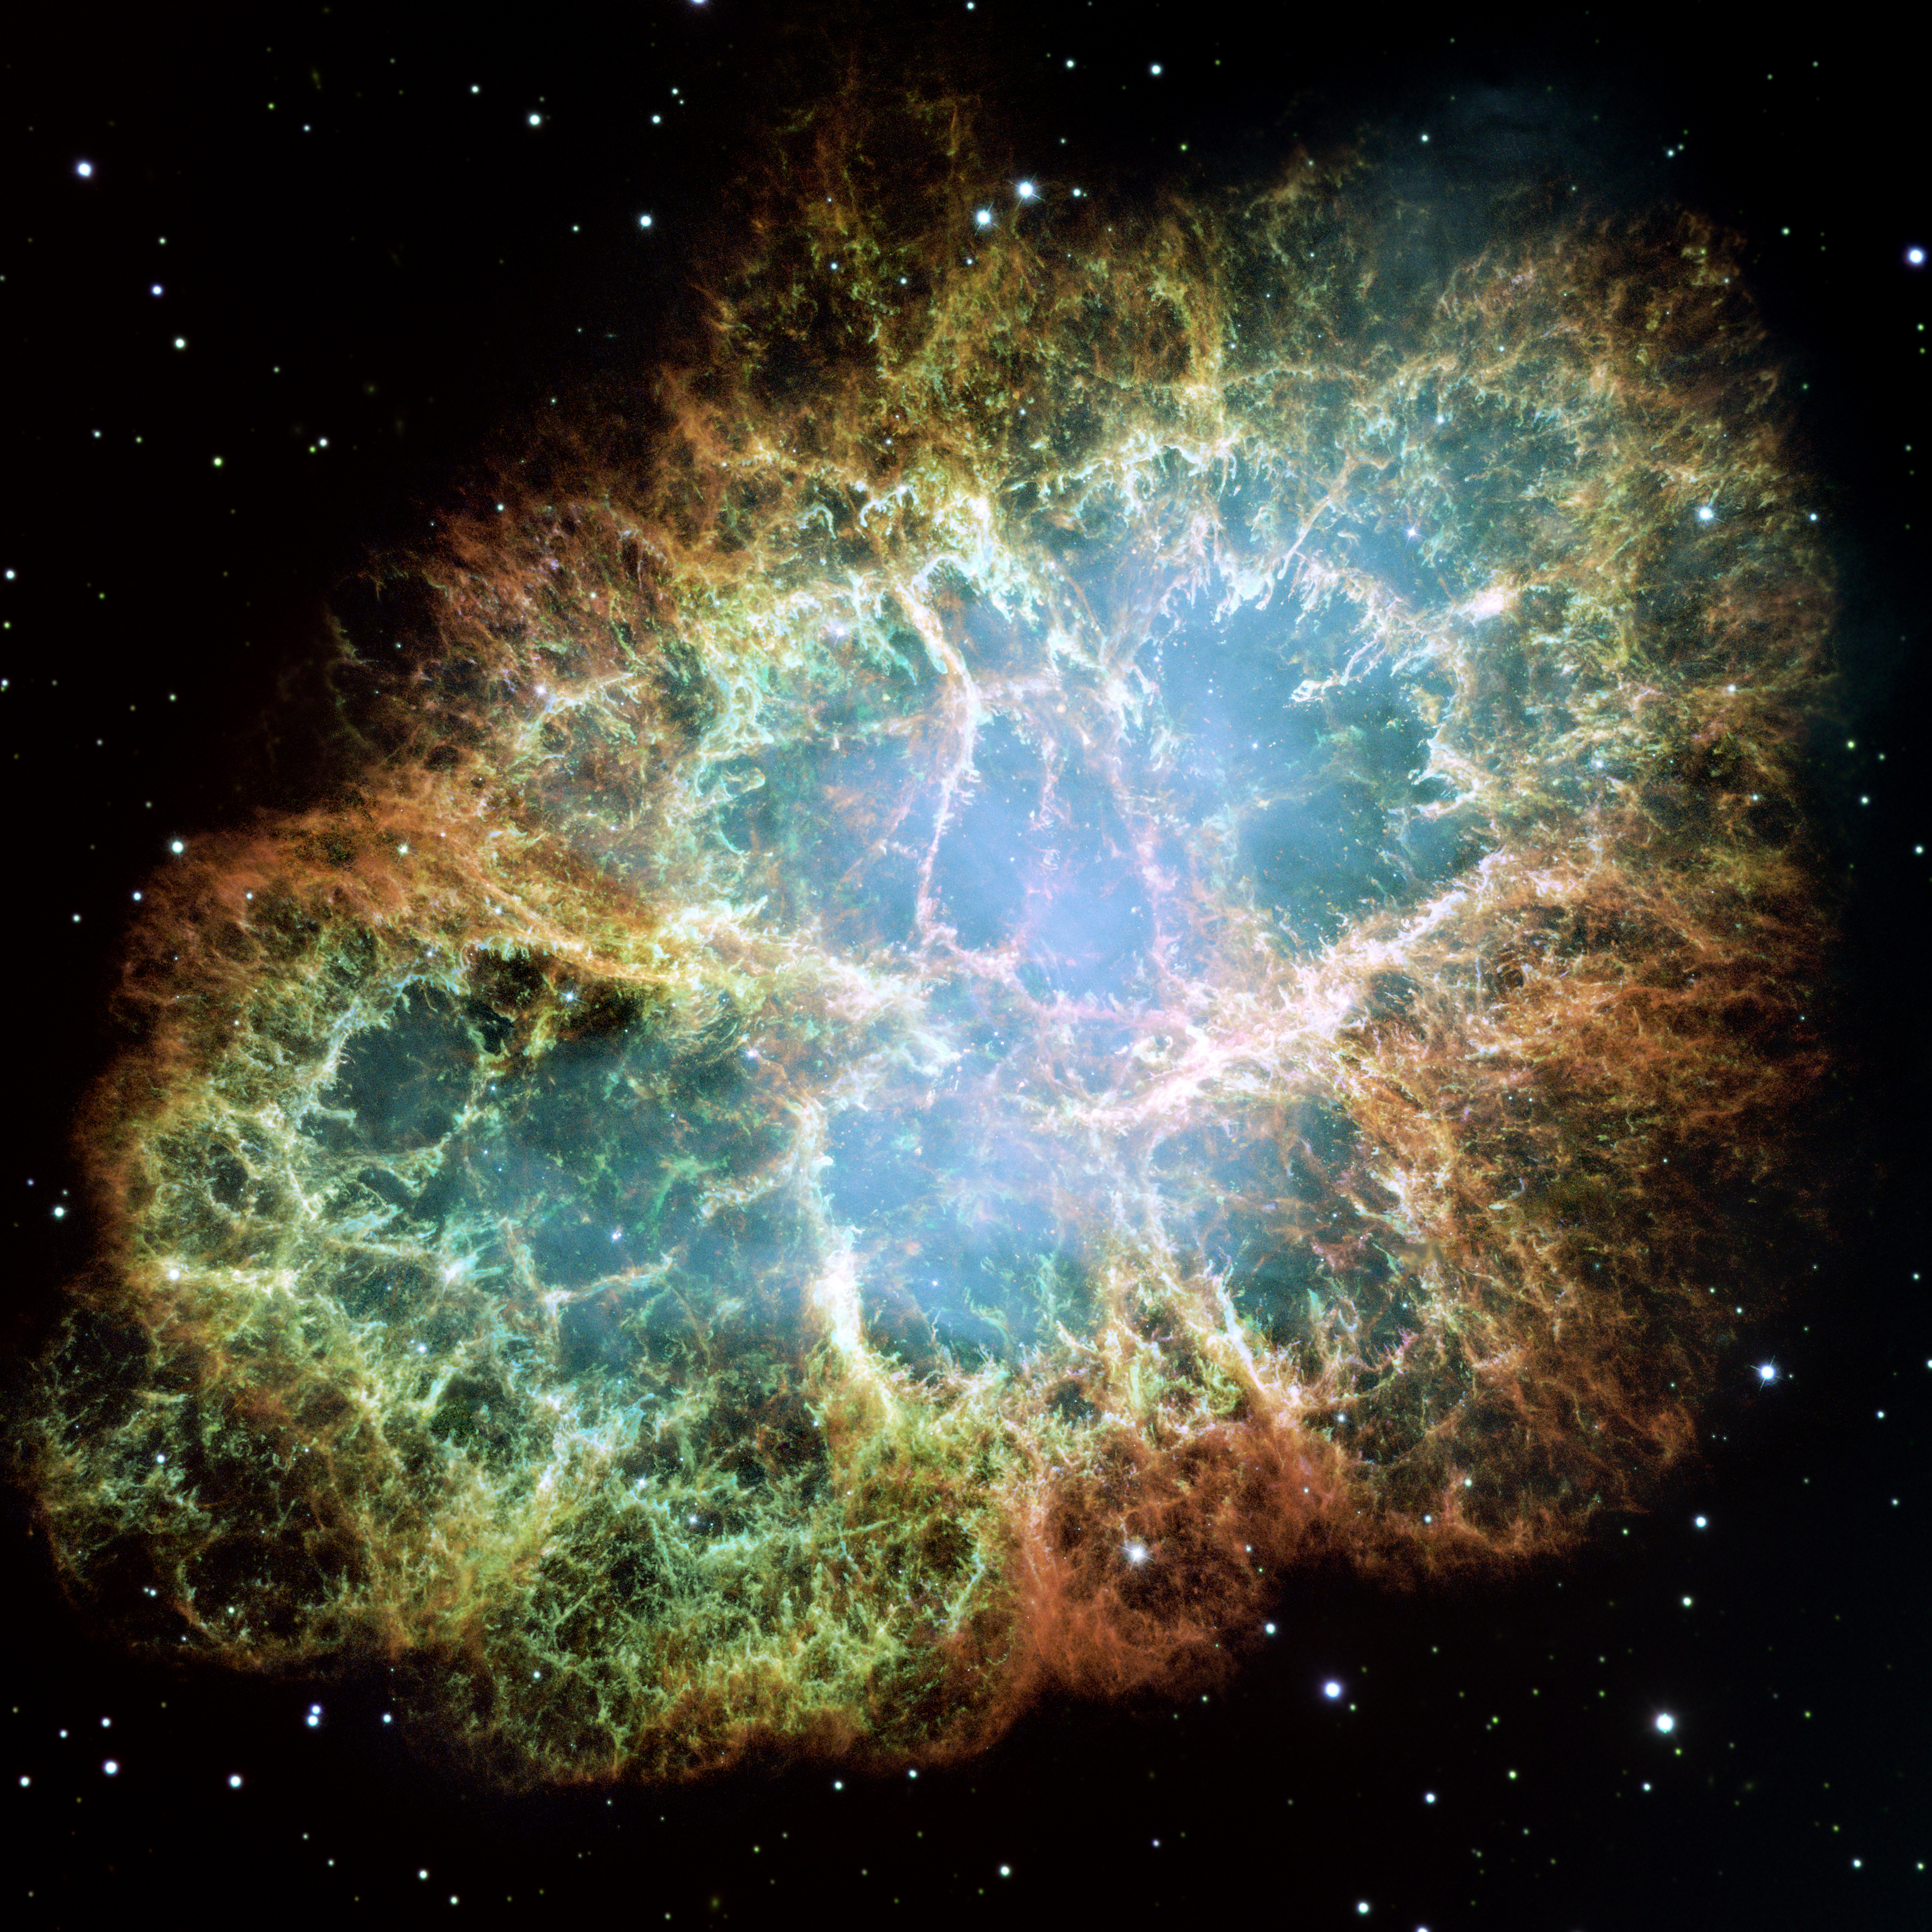
\includegraphics[width=1\textwidth]{Crab_Nebula.jpg}
  \caption{The Crab Nebula, a typical example of stars much larger than our sun would end up as.}
  \label{fig:crabneb}
\end{subfigure}
\caption{The gases leftover from the death of stars look something like this}
\label{fig:crab+ring}
\end{figure}
\paragraph{What happens to stars with core mass $\leq$ 1.4\solmas?}
\paragraph{}
Now, as we had mentioned before, during the star's life, the majority of time that it spends is within the main sequence, during this time, the star burns only hydrogen, and assuming a homogeneous star, we would have hydrogen burning at the core. Now, as this star ages, the amount of helium at it's core increases since hydrogen (through several intermediate steps of fusion) fuses to a stable helium nuclei, however the amount of energy produced through hydrogen fusing isn't enough for helium to fuse, hence the helium just piles up at the core. Now, when this happens, the star eventually starts to bloat. Why you might ask, well, I am not sure myself hence would like to discuss this in person. 
\paragraph{}
However, after the hydrogen burns, the star, eventually starts burning helium, since now, when enough helium has accumulated within the core, the pressure at the core has become high enough to burn helium, which then burns into carbon and then into oxygen, however this is capped in this case with the mass of the star, since the core isn't massive enough, it cannot burn anything further than oxygen (or even carbon in some cases) and hence once it starts burning helium to carbon and oxygen, the radiation pressure (pressure created by the huge amounts of light emitted) pushes the outer shells away from the star. Hence this is what forms a \textbf{Planetary Nebulae}, i.e. a gas cloud remains of a star. These slowly dissipate into the surrounding space and hence form a shell around the star. A good example of this would be the ring nebulae. as shown. These kind of stars are the most common kind of stars and generally inhabit $\geq$90\% of the stars in the milky way, so it would be safe to say that whatever star you look at at any given time is probably a star that would one day end up as a planetary nebulae. 
\paragraph{What happens to the stars with core mass $\geq$ 1.4\solmas?}
\paragraph{}
This is where we come into the exclusive high mass star class. Stars with such massive cores are generally several tens of \solmas or even more. One of the most common example of the same would be Betelgeuse, a star that we look at almost every-time we have an observation. This star is one of the biggest stars in we see, to give you an idea as to how big this is, say we were to replace this with our sun, it's size would go all the way to the asteroid belt, and we would be having this conversation within it, that is, our molecules would not exist. This star is at the later stages of it's evolution and could go boom any day now and when it does, it would form a Neutron Star, however, the remnant would be quite interesting since, when that light reaches us, we would see another sun appear in the sky, yeah, it would be that bright. However, once that subsides, we would see something like the crab nebula in it's place (after fast forwarding a few thousand years). 
\paragraph{}
Now, based on what we discussed previously about the elements that form within the core of massive stars, when they run out of fuel, and collapse, the outer layers of the star explode in what is called a \textbf{Supernovae}, this is where all the elements heavier than Iron form. Take a minute and think about it, some of the elements in our body are their only because there was some star, in the distant past, so big that it stretches all the way to the asteroid belt, that, at the end stages of it's life, went unstable, and in a cataclysmic explosion spread it's enriched guts all over space, which then led to the formation of our sun, and a tiny little blue marble around it which then has you in it, reading and wondering about itself.




\newpage
\clearpage
\begin{thebibliography}{300}

\bibitem{ARC}
Choudhuri, Arnab Rai. Astrophysics for Physicists. Cambridge University Press, 2014.

\bibitem{BasuIntro}
Basu, Baidyanath, et al. An Introduction to Astrophysics. Prentice Hall International, 2013.

\bibitem{WhichwayQueen}
“Which Way Queen Of The Night?” Astro Bob, 22 Mar. 2009, astrobob.areavoices.com/2009/03/22/which-way-queen-of-the-night/.

\bibitem{WinterCircle}
“You Absolutely Must See The Winter Hexagon Tonight.” Astro Bob, 18 Jan. 2013, astrobob.areavoices.com/2013/01/17/you-must-absolutely-see-the-winter-hexagon-tonight/.

\bibitem{Cassi}
“Interesting Facts about the Constellation Cassiopeia.” Astronomy Trek - Astronomy News \& Reviews, 16 Feb. 2018, www.astronomytrek.com/interesting-facts-about-the-constellation-cassiopeia/.

\bibitem{Andro}
Westlake/Courtesy, Jimmy. “Jimmy Westlake: Andromeda vs. The Milky Way.” Steamboat Pilot Today, 6 Oct. 2017, www.steamboatpilot.com/news/jimmy-westlake-andromeda-vs-the-milky-way/.

\bibitem{Persi}
“Star-Splitters.” StarSplitters, bestdoubles.wordpress.com/category/4-choose-a-constellation/perseus/.

\bibitem{Pegasi}
“Star Constellation Facts: Pegasus, the Winged Horse.” Astronomy Trek - Astronomy News \& Reviews, 16 Nov. 2017, www.astronomytrek.com/exploring-the-constellation-pegasus/.

\bibitem{Tauri}
Wikipedia contributors. "Taurus (constellation)." Wikipedia, The Free Encyclopedia. Wikipedia, The Free Encyclopedia, 11 Oct. 2018. Web. 12 Oct. 2018.

\bibitem{Orion}
“Orion the Hunter Now Easy to View.” EarthSky, earthsky.org/?p=13996.

\bibitem{CM}
“Interesting Facts About The Constellation Canis Major.” Astronomy Trek - Astronomy News \& Reviews, 19 Feb. 2018, www.astronomytrek.com/interesting-facts-about-the-constellation-canis-major/.

\bibitem{Gem}
Mathisen, David Warner. “Gemini, Canis Minor and the Hairy Twin.” The Mathisen Corollary, 1 Jan. 1970, mathisencorollary.blogspot.com/2011/06/gemini-canis-minor-and-hairy-twin.html.

\bibitem{Leo}
Lehr, Paul. “Hebrew Mazzaroth, Arranged by Phil Kulis.” God in a Nutshell Project, 16 Aug. 2018, godinanutshell.com/2018/08/15/hebrew-mazzaroth-arranged-phil-kulis/.

\bibitem{Planets_1}
Bryner, Jeanna. “The Storied History of the Word 'Planet'.” Space.com, Space.com, 8 Mar. 2016, www.space.com/5743-storied-history-word-planet.html.

\bibitem{wiki_planet_round}
Wikipedia contributors. "Spherical Earth." Wikipedia, The Free Encyclopedia. Wikipedia, The Free Encyclopedia, 22 Aug. 2018. Web. 23 Aug. 2018.

\bibitem{OTSOG}
Hawking, Stephen. On the Shoulders of Giants: the Great Works of Physics and Astronomy. Running Press, 2002.

\bibitem{AASP}
Strous, Louis. “Ask A Solar Physicist FAQs - Answer.” Stanford Solar Center, solar-center.stanford.edu/FAQ/Qsunasstar.html.

\bibitem{ASHistory}
“Spectroscopy and the Birth of Astrophysics (Cosmology: Tools).” The Discovery of Global Warming - A History, Center for History of Physics, history.aip.org/exhibits/cosmology/tools/tools-spectroscopy.htm

\bibitem{wiki_constellation}
Wikipedia contributors. "Constellation." Wikipedia, The Free Encyclopedia. Wikipedia, The Free Encyclopedia, 19 Aug. 2018. Web. 25 Aug. 2018.

\bibitem{constellationsHist}
Rao, Joe. “How the Night Sky Constellations Got Their Names.” Space.com, Space.com, 8 Mar. 2016, www.space.com/15486-night-sky-constellations-names.html.

\bibitem{astrometry_wiki}
Wikipedia contributors. "Astrometry." Wikipedia, The Free Encyclopedia. Wikipedia, The Free Encyclopedia, 21 Aug. 2018. Web. 25 Aug. 2018.

\bibitem{azimuth_wiki}
Wikipedia contributors. "Azimuth." Wikipedia, The Free Encyclopedia. Wikipedia, The Free Encyclopedia, 27 Jul. 2018. Web. 26 Aug. 2018.

\bibitem{coord_wiki}
Wikipedia contributors. "Celestial coordinate system." Wikipedia, The Free Encyclopedia. Wikipedia, The Free Encyclopedia, 20 Aug. 2018. Web. 26 Aug. 2018.

\bibitem{equi_coord1}
“Equatorial Coordinate System | COSMOS.” 7, astronomy.swin.edu.au/cosmos/E/Equatorial Coordinate System.

\bibitem{equi_coord2}
“Celestial Coordinate System.” Classification of the Planets, \\www.pas.rochester.edu/~blackman/ast104/coordinates.html.

\bibitem{precession1}
“The Precession of the Earth's Axis.” Structure of a Black Hole, \\astrosun2.astro.cornell.edu/academics/courses/astro201/earth\_precess.htm.

\bibitem{precession2}
“The Earth's Wobble – Precession.” My Dark Sky, 14 Oct. 2008, mydarksky.org/2008/10/14/the-earths-wobble-precession/.

\bibitem{precession3}
“Astronomy: Precession of Earth.” Astronomy: Greek Astronomy, astro.wsu.edu/worthey/astro/html/lec-precession.html.

\bibitem{epoch1}
Wikipedia contributors. "Epoch (astronomy)." Wikipedia, The Free Encyclopedia. Wikipedia, The Free Encyclopedia, 6 Aug. 2018. Web. 30 Aug. 2018.

\bibitem{epoch2}
Wilkins, D.R., and S.J. Crass. “J1950 And J2000 Epochs.” Stellar Mass and Supermassive Black Holes | Institute of Astronomy, Institute of Astronomy , www.ast.cam.ac.uk/public/ask/1960.

\bibitem{epoch3}
“Epoch | COSMOS.” 7, astronomy.swin.edu.au/cosmos/e/epoch.

\bibitem{epoch4}
Montenbruck, Oliver, and Thomas Pfleger. Astronomy on the Personal Computer. Springer Verlag, 2013.

\bibitem{newttele1}
Hall, Alfred Rupert. Isaac Newton: Adventurer in Thought. Univ. Press, 2000.

\bibitem{newttele2}
Wikipedia contributors. "Newtonian telescope." Wikipedia, The Free Encyclopedia. Wikipedia, The Free Encyclopedia, 28 Jul. 2018. Web. 30 Aug. 2018.

\bibitem{Tele_form1}
Chuck Hawks. “Simple Formulas for the Telescope Owner.” Sky \& Telescope, 20 Nov. 2017, www.skyandtelescope.com/observing/stargazers-corner/simple-formulas-for-the-telescope-owner/.

\bibitem{TeleFOV}
Swanson, Mike. “Field of View in a Telescope.” Nexstarsite, Ryukyu Astronomy Club, www.nexstarsite.com/\_RAC/articles/fieldofview.htm.

\bibitem{AO1}
Wikipedia contributors. "Adaptive optics." Wikipedia, The Free Encyclopedia. Wikipedia, The Free Encyclopedia, 20 Jun. 2018. Web. 26 Sep. 2018.

\bibitem{Refractor1}
Wikipedia contributors. "Refracting telescope." Wikipedia, The Free Encyclopedia. Wikipedia, The Free Encyclopedia, 14 Sep. 2018. Web. 26 Sep. 2018.

\bibitem{ChromatAberration}
Wikipedia contributors. "Chromatic aberration." Wikipedia, The Free Encyclopedia. Wikipedia, The Free Encyclopedia, 25 Apr. 2018. Web. 1 Oct. 2018.

\bibitem{CataTele}
Wikipedia contributors. "Catadioptric system." Wikipedia, The Free Encyclopedia. Wikipedia, The Free Encyclopedia, 9 Jul. 2018. Web. 10 Oct. 2018.

\bibitem{AO1}
Wikipedia contributors. "Adaptive optics." Wikipedia, The Free Encyclopedia. Wikipedia, The Free Encyclopedia, 2 Oct. 2018. Web. 10 Oct. 2018.

\bibitem{AO2}
information@eso.org. “Adaptive Optics.” ESO, www.eso.org/public/teles-instr/technology/adaptive\_optics/. 

\bibitem{AO3}
Sky $\&$ Telescope. “Adaptive Optics: Before and After.” Sky $\&$ Telescope, Sky $\&$ Telescope, 21 Mar. 2016, www.skyandtelescope.com/sky-and-telescope-magazine/beyond-the-printed-page/adaptive-optics-before-and-after/.

\bibitem{Parallax}
Wikipedia contributors. "Stellar parallax." Wikipedia, The Free Encyclopedia. Wikipedia, The Free Encyclopedia, 30 Sep. 2018. Web. 11 Oct. 2018.

\bibitem{StellarMag}
Wikipedia contributors. "Magnitude (astronomy)." Wikipedia, The Free Encyclopedia. Wikipedia, The Free Encyclopedia, 16 Sep. 2018. Web. 11 Oct. 2018.

\bibitem{DistLadder1}
Wikipedia contributors. "Cosmic distance ladder." Wikipedia, The Free Encyclopedia. Wikipedia, The Free Encyclopedia, 19 Sep. 2018. Web. 11 Oct. 2018.

\bibitem{DistLadder2}
Darling, David. “Cosmic Distance Ladder.” The Worlds of David Darling, www.daviddarling.info/encyclopedia/C/cosmic\_distance\_ladder.html.

\bibitem{Wiki_CMB}
Wikipedia contributors. "Cosmic microwave background." Wikipedia, The Free Encyclopedia. Wikipedia, The Free Encyclopedia, 14 Feb. 2019. Web. 27 Feb. 2019.

\bibitem{reionisation1}
Asu. “Unlocking the Secrets of the Universe.” EurekAlert!, www.eurekalert.org/pub\_releases/2018-02/asu-uts022618.php.

\bibitem{HRD}
Wikipedia contributors. "Hertzsprung–Russell diagram." Wikipedia, The Free Encyclopedia. Wikipedia, The Free Encyclopedia, 26 Feb. 2019. Web. 1 Mar. 2019.

\bibitem{HayashiHenny}
Wikipedia contributors. "Hayashi track." Wikipedia, The Free Encyclopedia. Wikipedia, The Free Encyclopedia, 16 Mar. 2018. Web. 1 Mar. 2019.

\bibitem{Joshi1}
Joshi, Pankaj S. The Story of Collapsing Stars: Black Holes, Naked Singularities, and the Cosmic Play of Quantum Gravity. Oxford University Press, 2018.


\end{thebibliography}
\end{document}

